% Options for packages loaded elsewhere
\PassOptionsToPackage{unicode}{hyperref}
\PassOptionsToPackage{hyphens}{url}
\PassOptionsToPackage{dvipsnames,svgnames,x11names}{xcolor}
%
\documentclass[
  12pt,
  letterpaper,
  DIV=11,
  numbers=noendperiod]{scrreprt}

\usepackage{amsmath,amssymb}
\usepackage{iftex}
\ifPDFTeX
  \usepackage[T1]{fontenc}
  \usepackage[utf8]{inputenc}
  \usepackage{textcomp} % provide euro and other symbols
\else % if luatex or xetex
  \usepackage{unicode-math}
  \defaultfontfeatures{Scale=MatchLowercase}
  \defaultfontfeatures[\rmfamily]{Ligatures=TeX,Scale=1}
\fi
\usepackage{lmodern}
\ifPDFTeX\else  
    % xetex/luatex font selection
\fi
% Use upquote if available, for straight quotes in verbatim environments
\IfFileExists{upquote.sty}{\usepackage{upquote}}{}
\IfFileExists{microtype.sty}{% use microtype if available
  \usepackage[]{microtype}
  \UseMicrotypeSet[protrusion]{basicmath} % disable protrusion for tt fonts
}{}
\makeatletter
\@ifundefined{KOMAClassName}{% if non-KOMA class
  \IfFileExists{parskip.sty}{%
    \usepackage{parskip}
  }{% else
    \setlength{\parindent}{0pt}
    \setlength{\parskip}{6pt plus 2pt minus 1pt}}
}{% if KOMA class
  \KOMAoptions{parskip=half}}
\makeatother
\usepackage{xcolor}
\usepackage[a4paper]{geometry}
\setlength{\emergencystretch}{3em} % prevent overfull lines
\setcounter{secnumdepth}{5}
% Make \paragraph and \subparagraph free-standing
\makeatletter
\ifx\paragraph\undefined\else
  \let\oldparagraph\paragraph
  \renewcommand{\paragraph}{
    \@ifstar
      \xxxParagraphStar
      \xxxParagraphNoStar
  }
  \newcommand{\xxxParagraphStar}[1]{\oldparagraph*{#1}\mbox{}}
  \newcommand{\xxxParagraphNoStar}[1]{\oldparagraph{#1}\mbox{}}
\fi
\ifx\subparagraph\undefined\else
  \let\oldsubparagraph\subparagraph
  \renewcommand{\subparagraph}{
    \@ifstar
      \xxxSubParagraphStar
      \xxxSubParagraphNoStar
  }
  \newcommand{\xxxSubParagraphStar}[1]{\oldsubparagraph*{#1}\mbox{}}
  \newcommand{\xxxSubParagraphNoStar}[1]{\oldsubparagraph{#1}\mbox{}}
\fi
\makeatother


\providecommand{\tightlist}{%
  \setlength{\itemsep}{0pt}\setlength{\parskip}{0pt}}\usepackage{longtable,booktabs,array}
\usepackage{calc} % for calculating minipage widths
% Correct order of tables after \paragraph or \subparagraph
\usepackage{etoolbox}
\makeatletter
\patchcmd\longtable{\par}{\if@noskipsec\mbox{}\fi\par}{}{}
\makeatother
% Allow footnotes in longtable head/foot
\IfFileExists{footnotehyper.sty}{\usepackage{footnotehyper}}{\usepackage{footnote}}
\makesavenoteenv{longtable}
\usepackage{graphicx}
\makeatletter
\newsavebox\pandoc@box
\newcommand*\pandocbounded[1]{% scales image to fit in text height/width
  \sbox\pandoc@box{#1}%
  \Gscale@div\@tempa{\textheight}{\dimexpr\ht\pandoc@box+\dp\pandoc@box\relax}%
  \Gscale@div\@tempb{\linewidth}{\wd\pandoc@box}%
  \ifdim\@tempb\p@<\@tempa\p@\let\@tempa\@tempb\fi% select the smaller of both
  \ifdim\@tempa\p@<\p@\scalebox{\@tempa}{\usebox\pandoc@box}%
  \else\usebox{\pandoc@box}%
  \fi%
}
% Set default figure placement to htbp
\def\fps@figure{htbp}
\makeatother
% definitions for citeproc citations
\NewDocumentCommand\citeproctext{}{}
\NewDocumentCommand\citeproc{mm}{%
  \begingroup\def\citeproctext{#2}\cite{#1}\endgroup}
\makeatletter
 % allow citations to break across lines
 \let\@cite@ofmt\@firstofone
 % avoid brackets around text for \cite:
 \def\@biblabel#1{}
 \def\@cite#1#2{{#1\if@tempswa , #2\fi}}
\makeatother
\newlength{\cslhangindent}
\setlength{\cslhangindent}{1.5em}
\newlength{\csllabelwidth}
\setlength{\csllabelwidth}{3em}
\newenvironment{CSLReferences}[2] % #1 hanging-indent, #2 entry-spacing
 {\begin{list}{}{%
  \setlength{\itemindent}{0pt}
  \setlength{\leftmargin}{0pt}
  \setlength{\parsep}{0pt}
  % turn on hanging indent if param 1 is 1
  \ifodd #1
   \setlength{\leftmargin}{\cslhangindent}
   \setlength{\itemindent}{-1\cslhangindent}
  \fi
  % set entry spacing
  \setlength{\itemsep}{#2\baselineskip}}}
 {\end{list}}
\usepackage{calc}
\newcommand{\CSLBlock}[1]{\hfill\break\parbox[t]{\linewidth}{\strut\ignorespaces#1\strut}}
\newcommand{\CSLLeftMargin}[1]{\parbox[t]{\csllabelwidth}{\strut#1\strut}}
\newcommand{\CSLRightInline}[1]{\parbox[t]{\linewidth - \csllabelwidth}{\strut#1\strut}}
\newcommand{\CSLIndent}[1]{\hspace{\cslhangindent}#1}

\usepackage{makeidx}
\makeindex
\KOMAoption{captions}{tableheading}
\makeatletter
\@ifpackageloaded{bookmark}{}{\usepackage{bookmark}}
\makeatother
\makeatletter
\@ifpackageloaded{caption}{}{\usepackage{caption}}
\AtBeginDocument{%
\ifdefined\contentsname
  \renewcommand*\contentsname{Table of contents}
\else
  \newcommand\contentsname{Table of contents}
\fi
\ifdefined\listfigurename
  \renewcommand*\listfigurename{List of Figures}
\else
  \newcommand\listfigurename{List of Figures}
\fi
\ifdefined\listtablename
  \renewcommand*\listtablename{List of Tables}
\else
  \newcommand\listtablename{List of Tables}
\fi
\ifdefined\figurename
  \renewcommand*\figurename{Figure}
\else
  \newcommand\figurename{Figure}
\fi
\ifdefined\tablename
  \renewcommand*\tablename{Table}
\else
  \newcommand\tablename{Table}
\fi
}
\@ifpackageloaded{float}{}{\usepackage{float}}
\floatstyle{ruled}
\@ifundefined{c@chapter}{\newfloat{codelisting}{h}{lop}}{\newfloat{codelisting}{h}{lop}[chapter]}
\floatname{codelisting}{Listing}
\newcommand*\listoflistings{\listof{codelisting}{List of Listings}}
\makeatother
\makeatletter
\makeatother
\makeatletter
\@ifpackageloaded{caption}{}{\usepackage{caption}}
\@ifpackageloaded{subcaption}{}{\usepackage{subcaption}}
\makeatother

\usepackage{bookmark}

\IfFileExists{xurl.sty}{\usepackage{xurl}}{} % add URL line breaks if available
\urlstyle{same} % disable monospaced font for URLs
\hypersetup{
  pdftitle={Literaturgeschichte als Wissensgraph},
  pdfauthor={Julia Röttgermann},
  colorlinks=true,
  linkcolor={blue},
  filecolor={Maroon},
  citecolor={Blue},
  urlcolor={Blue},
  pdfcreator={LaTeX via pandoc}}


\title{Literaturgeschichte als Wissensgraph}
\usepackage{etoolbox}
\makeatletter
\providecommand{\subtitle}[1]{% add subtitle to \maketitle
  \apptocmd{\@title}{\par {\large #1 \par}}{}{}
}
\makeatother
\subtitle{Automatische Erhebung literaturhistorisch relevanter
Informationen aus Volltexten am Beispiel von französischen Romanen des
XVIII. Jahrhunderts}
\author{Julia Röttgermann}
\date{2025-04-08}

\begin{document}
\maketitle

\renewcommand*\contentsname{Table of contents}
{
\hypersetup{linkcolor=}
\setcounter{tocdepth}{2}
\tableofcontents
}

\bookmarksetup{startatroot}

\chapter*{Preface}\label{preface}
\addcontentsline{toc}{chapter}{Preface}

\markboth{Preface}{Preface}

This is a Quarto book.

To learn more about Quarto books visit
\url{https://quarto.org/docs/books}.

\bookmarksetup{startatroot}

\chapter{\texorpdfstring{\textbf{Stilometrische Analyse von
Französischen Romanen
1751-1800}}{Stilometrische Analyse von Französischen Romanen 1751-1800}}\label{stilometrische-analyse-von-franzuxf6sischen-romanen-1751-1800}

\begin{quote}
The close reader sees things in a text --- single moments and large
amorphous movements ---to which computer programs give no easy access.
The computer, on the other hand, reveals hidden patterns and enables us
to marshal hosts of instances too numerous for our unassisted powers.
\end{quote}

\begin{quote}
--- Burrows (2002); pp.~696
\end{quote}

\section{Einleitung: Was ist
Stilometrie?}\label{einleitung-was-ist-stilometrie}

Was ist Stilometrie und wozu können wir die Methode hinsichtlich einer
datenbasierten Literaturgeschichte einsetzen? Die Methode, die Anwendung
sowohl in den Digitalen Geisteswissenschaften als auch in der
forensischen Linguistik findet, nutzt linguistische Merkmale,
statistische Modelle, und computergestützte Verfahren, um stilistische
Muster in schriftlichen Texten zu identifizieren und zu vergleichen.
Eines der meist verbreiteten Ziele der Stilometrie\index{Stilometrie}
ist es dabei, die Autorschaft eines Textes mit computationellen Mitteln
nachzuweisen (Burrows 2002; Hoover 2010; Rotari / Jander / Rybicki
2021). Daneben gibt es jedoch auch Studien, die die statistischen
sprachlichen Eigenschaften hinsichtlich von Gender-Unterschieden,
Phänomene wie die individuellen Veränderungen eines Schreibstils im
Laufe der Zeit oder in unterschiedlichen literarischen Gattungen
analysieren (Holmes 1998; Jannidis / Lauer 2014; Schöch 2014; Weidman /
Pastor 2021).\\
Der Begriff Stilometrie setzt sich aus den beiden Wortteilen ``Stil''
und ``-metrie'' zusammen, also eine literarische oder linguistische
Kategorie (Stil) und das Konfix ``-metrie'', das suggeriert, dass etwas
gezählt wird.\footnote{Morozov (1854-1946) verwendet erstmals den
  Begriff ‚stilometrija /\emph{Stilometrie}` in Russland {[}Köhler /
  Altmann / Piotrowski (2005); pp.~37 ff.{]}. Für eine allgemeine
  Einführung in die Methode der Stilometrie im Kontext der Digital
  Humanities cf. (Laramée 2018; Horstmann 2024; Eder / Rybicki /
  Kestemont 2016).} Zunächst stellt sich daher die Frage: Was ist Stil?
Dazu haben (Herrmann / Van Dalen-Oskam / Schöch 2015) eine Definition
formuliert, die man sowohl für computationelle Methoden als auch im
klassischen literaturwissenschaftlichen Sinne anwenden kann: ``Style is
a property of texts constituted by an ensemble of formal features which
can be observed quantitatively or qualitatively'' (Herrmann / Van
Dalen-Oskam / Schöch 2015). Stilometrie nutzt das Zählen stilistischer
Merkmale in Form der Verwendungshäufigkeit bestimmter Wörter (`most
frequent words'), um Aussagen zur Textähnlichkeit zu generieren, die
unter bestimmten Bedingungen Rückschlüsse auf die Autorschaft
zulassen.\footnote{Hinzufügen könnte man außerdem, dass der Computer
  hier völlig neue Möglichkeiten eröffnete. Gingen Mosteller und Wallace
  in Teilen ihrer Berechnung noch händisch vor, ist es heute eine
  Selbstverständlichkeit, eine stilometrische Studie von einem Computer
  berechnen zu lassen. ``The most important technological advances in
  authorship studies have arisen from the computer.'' stellen sie auch
  selbst 20 Jahre nach ihrer wegweisenden Studie in einem Zusatzkapitel
  fest {[}Mosteller / Wallace (1963); pp.~268{]}.}

Das vorliegende Kapitel beginnt damit, die Anfänge bzw. wegweisende
Studien der Stilometrie zu beschreiben. Als Pionierstudien der
Stilometrie werden die Studie zu den \emph{Federalist Papers} (Mosteller
/ Wallace 1963) und Burrow's Delta (Burrows 2002) zusammengefasst. Als
weitere theoretische Grundlage werden verschiedene Distanzmaße und zudem
die Relevanz des R-Pakets `stylo' innerhalb der Community der Digital
Humanities beschrieben.\\
Im Anschluss beschreibe ich einen konkreten Anwendungsfall. Dazu
untersuche ich eine Fallstudie zu einem Roman mit ungeklärter
Autorschaft aus der Textsammlung roman18 in mehreren Schritten:
Verwendung eines Subkorpus von roman18, Analyse mit um Texte eines
potentiellen Autors erweitertem Datensatz, Hierarchical Wards
Clustering, Bootstrap Consensus Tree. Eine überraschende Erkenntnis
liefert der Vergleich aus Clustering und numerischen Distanzwerten der
stilometrischen Analyse. Abschließend beschreibe und diskutiere ich die
Modellierung in Wikibase unter Verwendung von `ranks' und
SPARQL-Abfragen zu Gemeinsamkeiten stilometrisch naher Werke.

\emph{Keywords: Stilometrie, Federalist Papers, Delta, stylo,
Hierarchical Wards Clustering, Bootstrap Consensus Tree, Principal
Component Analysis, Wikibase, preferred rank, SPARQL.}

\section{Pionierstudien und
Toolentwicklung}\label{pionierstudien-und-toolentwicklung}

Eine Studie von Mosteller und Wallace 1964 zu den \emph{Federalist
Papers} verschaffte der Stilometrie den wissenschaftlichen Durchbruch:
Die \emph{Federalist Papers} sind eine 1787-1788 veröffentlichte
Sammlung von 85 Essays zur politischen Theorie. In diesen 900 bis 3500
Wörter langen Schriften, die während der Debatte über die Ratifizierung
der Verfassung der Vereinigten Staaten verfasst wurden, werden die
Argumente für das Regierungssystem dargelegt, dass die USA schließlich
angenommen haben und unter dem sie bis zum heutigen Tag leben. Die
Autorschaft dieser Artikel, unterzeichnet mit dem Pseudonym ``Publius'',
war lange Zeit unklar (Laramée 2018). Mithilfe der Analyse der
Wortfrequenzen gelang es Mosteller und Wallace, die ungeklärte Zuordnung
aus mehreren möglichen Autoren aufzulösen {[}Kenny (1982); pp.8--9{]}.
Die Bedingungen in der \emph{Federalist Paper}-Studie können sicherlich
auch als ideal gelten, werden doch mehrere Parameter - wie Kontext,
Gender und Gattung - konstant gehalten.

Ein weiterer bedeutender Beitrag zur Stilometrie stammt von John
Burrows, der das Distanzmaß ›Delta‹ entwickelte, mithilfe dessen sich
für einen anonymen Text eine Zuordnung zu einem Korpus bekannter Texte
und Autor:innen treffen lässt. Seine Studie, die multivariate
statistische Verfahren wie Cluster- oder Principal Component Analyse
(PCA) einsetzt, und die daraus resultierenden Erkenntnisse haben
bedeutende Impulse für die Stilometrie und die Autorschaftsattribution
in den Computational Literary Studies geliefert. Burrows Delta verwendet
den Manhattan-Abstand und hat sich als besonders effektiv erwiesen, um
Autorschaftsfragen oder die Beteiligung einzelner Autoren an
umfangreichen Textsammlungen zu klären (Büttner et al. 2017). Basierend
auf Burrows Delta wurden weitere Varianten zur Verbesserung
vorgeschlagen, beispielsweise der Vorschlag, statt der Manhattan-Distanz
den Kosinus-Winkel zwischen den Vektoren zu verwenden (Smith / Aldridge
2011).\footnote{Das Projekt ``\textbf{\emph{Zeta und Konsorten}.}
  Distinktivitätsmaße für die Computational Literary Studies.`` am Trier
  Center for Digital Humanities hat es sich zum Ziel gesetzt, ein
  tieferes Verständnis verschiedener Distinktivitätsmaße zu erreichen
  und Verbesserungen in deren Implementierung und Anwendung
  vorzuschlagen (cf. Du / Dudar / Schöch 2022).}

Bezüglich der Toolentwicklung kommt Maciej Eder, Jan Rybicki und Mike
Kestemont der Verdienst zu, ein eingängiges, leicht bedienbares Tool für
die Statistikumgebung R entwickelt zu haben, dass auch zur weiten
Verbreitung der Methode in den Digital Humanities und darüber hinaus
geführt hat (Horstmann 2024): ``Stylo'' (Eder / Rybicki / Kestemont
2016).

\section{Theoretische Grundlagen:
Distanzmaße}\label{theoretische-grundlagen-distanzmauxdfe}

\begin{figure}

\centering{

\pandocbounded{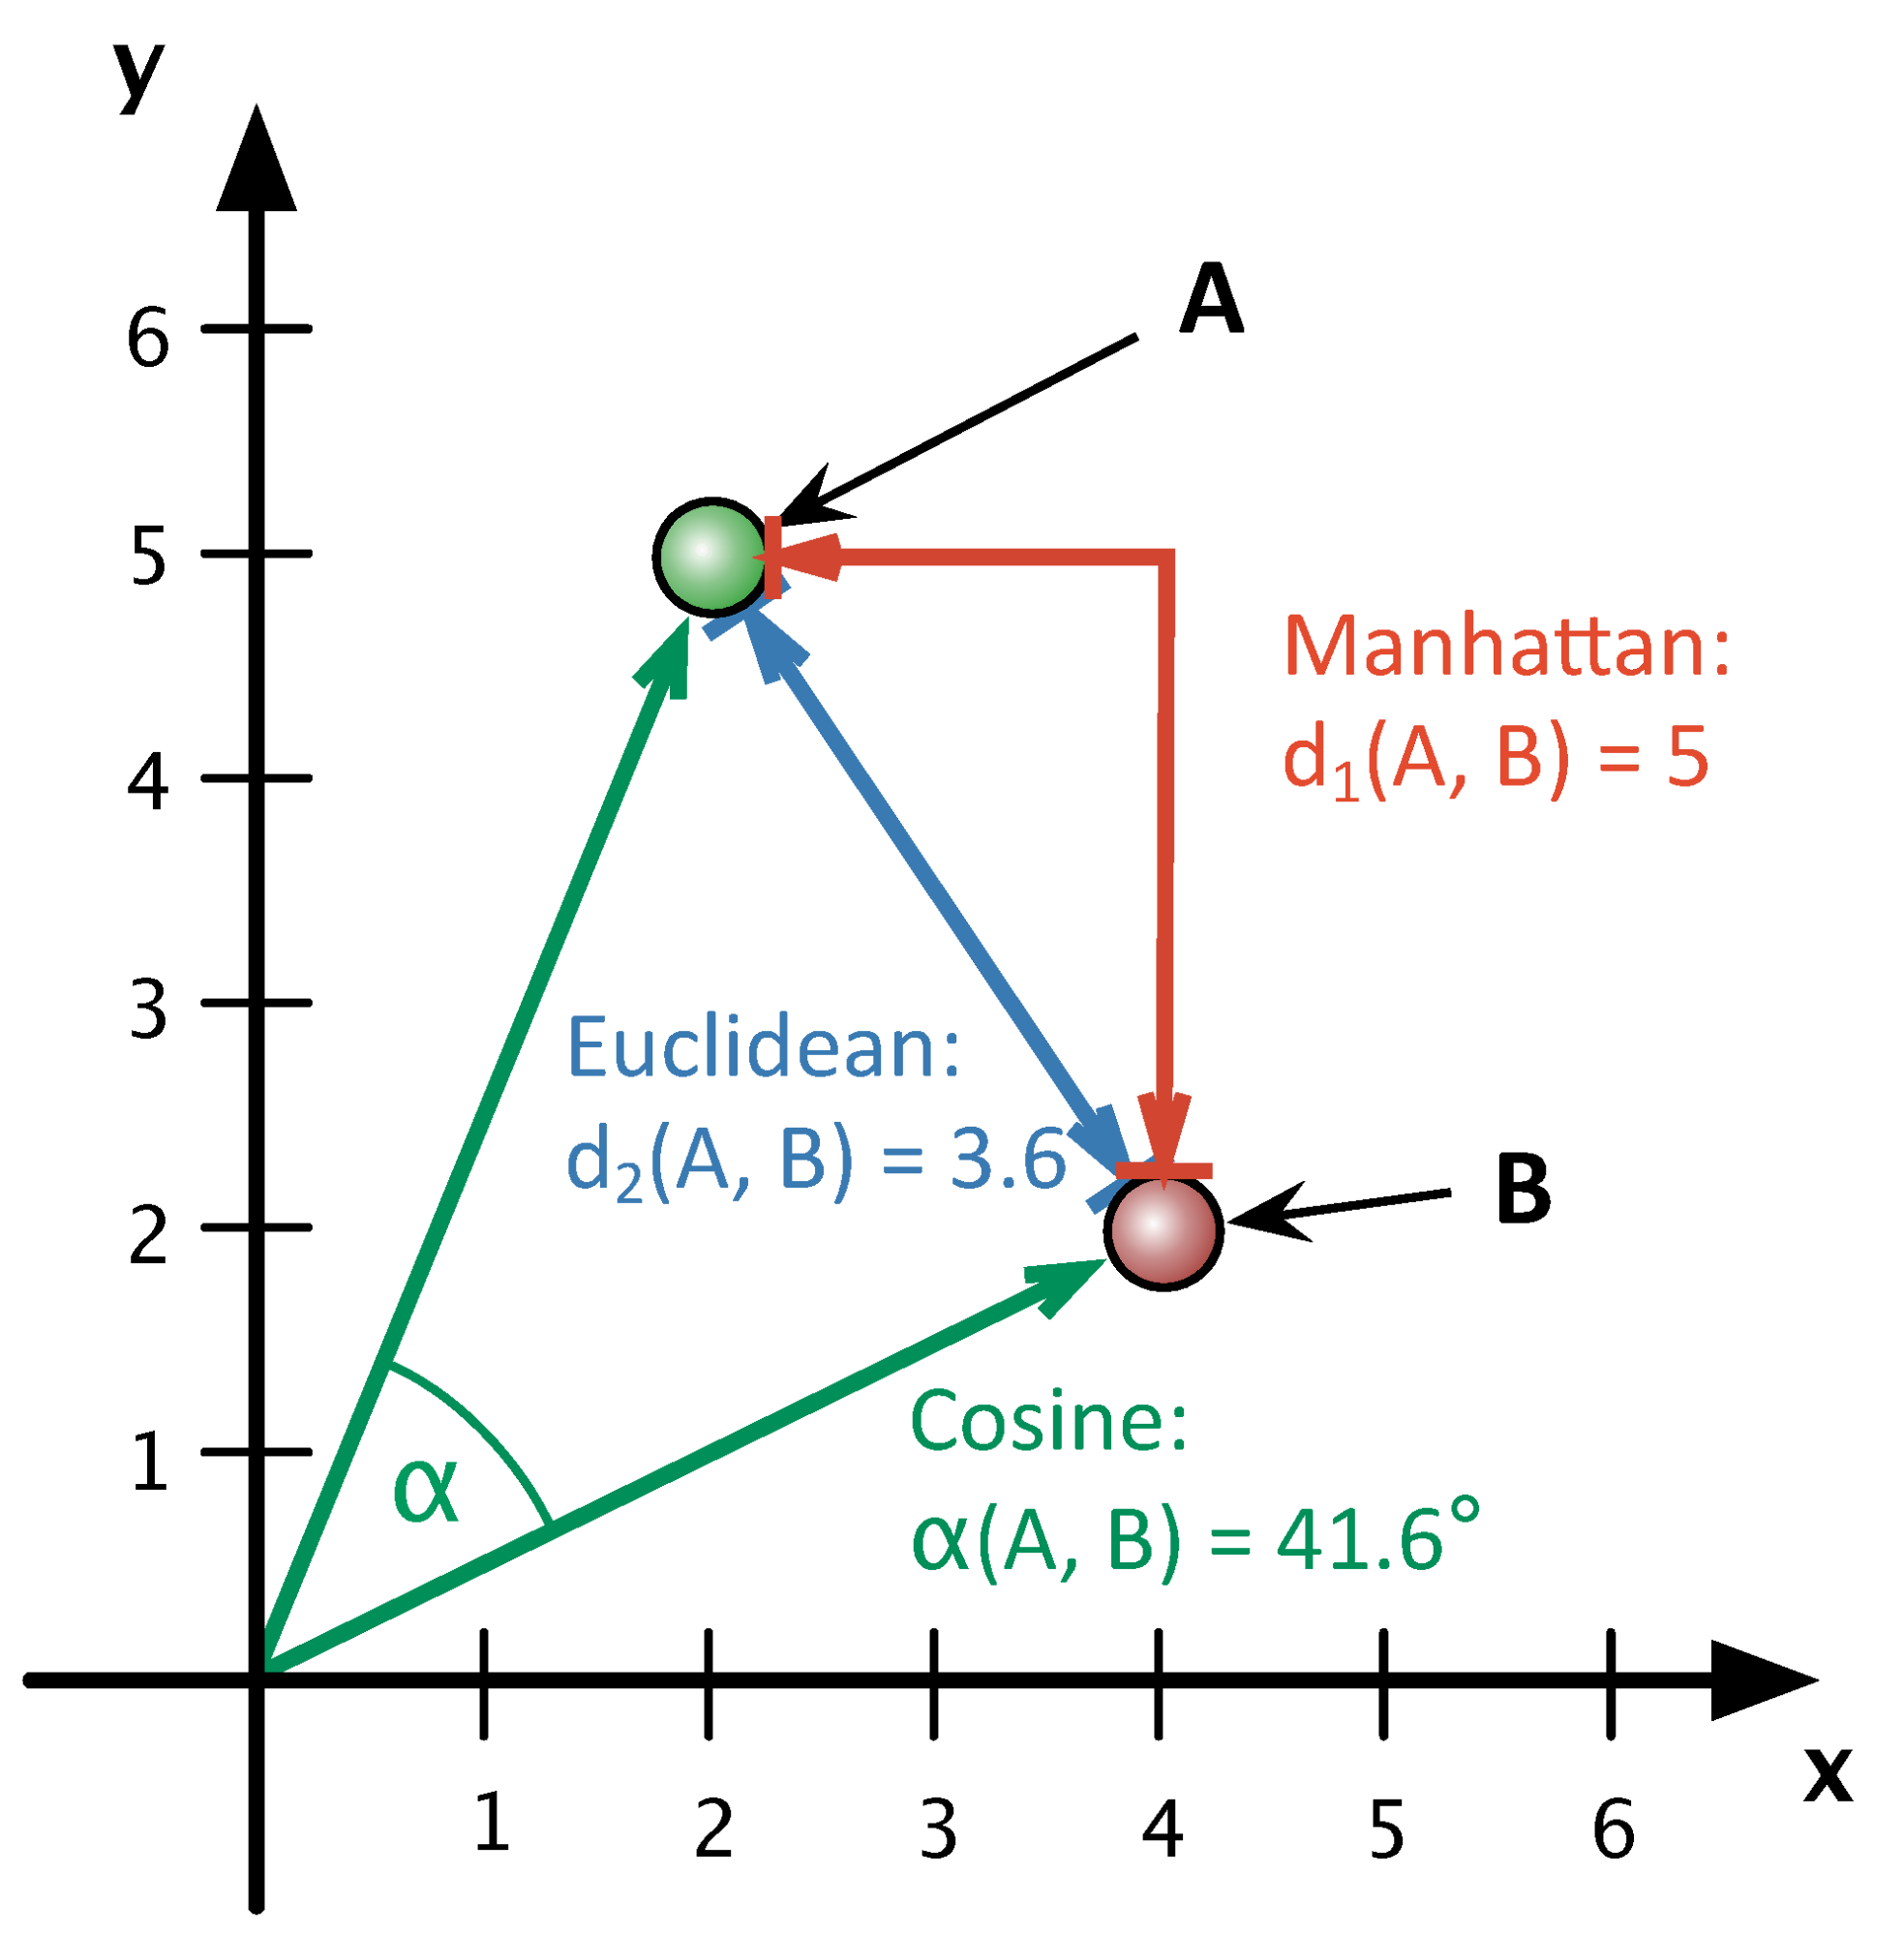
\includegraphics[keepaspectratio]{img_06/evert_jannidis_schoch_2016.png}}

}

\caption{\label{fig-distance-measures}Distanzmaße: Manhattan-Distanz,
Euklidische Distanz und Kosinus-Distanz {[}Stefan Evert, 2017.
Lizenziert unter Creative Commons Namensnennung 4.0 International
(CC-BY){]}}

\end{figure}%

Im Kontext der Textanalyse werden verschiedene Distanzmaße verwendet, um
die Unterschiede zwischen Texten zu quantifizieren {[}Schöch (2017);
pp.~294--295{]}. Die \textbf{Manhattan-Distanz} misst die absolute
Distanz zweier Vektoren in jeder einzelnen Dimension. Die Summe dieser
absoluten Distanzen ergibt die Gesamtdistanz, wobei jede Dimension
gleich gewichtet wird (Figure~\ref{fig-distance-measures}).

Die \textbf{Euklidische Distanz} ähnelt der Vogelfluglinie zwischen zwei
Punkten. Hierbei werden die Distanzen in jeder Dimension quadriert,
summiert und schließlich die Quadratwurzel aus der Gesamtsumme gezogen.
Dies führt dazu, dass größere Distanzen in einer einzelnen Dimension
durch die Quadrierung stärker gewichtet werden, was in der
stilometrischen Autorschaftsattribution besonders relevant ist, da
häufig vorkommende Wörter einen überproportionalen Einfluss haben
können. Bei der euklidischen Distanz haben die höchstfrequenten Wörter
besonders viel Einfluss.

Der \textbf{Kosinus-Abstand} wird als eine Form der
Vektor-Normalisierung betrachtet, da bei der Berechnung des Winkels
zwischen Vektoren die Länge der Vektoren keine Rolle spielt. Im
Gegensatz zu Manhattan- und Euklidischem Abstand ermöglicht der
Kosinus-Abstand eine Bewertung, die unabhängig von der Länge der
Vektoren ist.

In Bezug auf die stilometrische Autorschaftsattribution betonen (Büttner
et al. 2017), dass das charakteristische stilistische Profil eines
Autors eher in der qualitativen Kombination bestimmter Wortpräferenzen
zu finden ist. Dies bezieht sich auf das grundlegende Muster von über-
bzw. unterdurchschnittlich häufigem Gebrauch von Wörtern, anstatt auf
die Amplitude dieser Abweichungen. ``Delta'' in der stilometrischen
Autorschaftsattribution nutzt die Manhattan-Distanz und erweist sich als
erfolgreich, da es strukturelle Unterschiede in den sprachlichen
Vorlieben eines Autors erfasst, ohne stark von der Intensität des
Autorenprofils in einem bestimmten Text beeinflusst zu werden (Evert et
al. 2017).

Nachdem nun wegweisende Studien der Stilometrie vorgestellt und
theoretische Grundlagen der Methode erläutert wurden, stellt sich die
Frage, wozu stilometrische Analysen im Kontext einer datenbasierten
Literaturgeschichte beitragen können. Eine der häufigsten
Anwendungsfälle stellt sicherlich die Autorschaftsattribution dar. Ob J.
K. Rowling (Juola 2015) oder Shakespeare (Craig / Kinney 2009) lassen
sich hier viele Anwendungsstudien zitieren.\\
Stilometrie lässt sich jedoch neben der Analyse von Autorschaftssignalen
auch zur Bestimmung von Gattungszugehörigkeit einsetzen (Schöch 2014)
oder in der diachronen Betrachtung einer stilistischen Handschrift eines
einzelnen Autors oder Autorin, beispielsweise in der Frage: Gibt es so
etwas wie ``late style'' (Reeve; Rebora / Salgaro 2018)?

Wieso funktioniert die Methode Stilometrie? Dies lässt sich durch einen
interessanten historischen Vergleich in der kunsthistorischen Forschung
veranschaulichen, den Mike Kestemont beschreibt. Der Wechsel von
Inhaltswörtern zu Funktionswörtern in Studien zur
Autorschaftsattribution findet hier eine bemerkenswerte Parallele:

``Giovanni Morelli (1816-1891) was among the first to suggest that the
attribution of, for instance, a\\
Quattrocento painting to some Italian master, could not happen based on
`content' {[}\ldots{]} Morelli thought it better to restrict an
authorship analysis to discrete details such as ears, hands and
feet''~(Kestemont 2014: pp.61)

Auch in der Malerei lassen sich über die Analyse von unwillkürlich
getroffenen Entscheidungen, wie der Art, die Hände, Ohren oder Füße zu
malen, Rückschlüsse auf die Autorschaft ziehen. Das Zitat unterstreicht
die Faszination darüber, dass Menschen, sei es in Texten oder Gemälden,
unbewusste Entscheidungen treffen, die in der Summe Aufschlüsse über
ihre künstlerische Handschrift geben, so auch bei der Verwendung
bestimmter Funktionswörter.

Im nächsten Abschnitt sollen mithilfe von Stilometrie innerhalb des
Korpus französischer Romane 1751-1800 (roman18) Aussagen zur möglichen
Autorschaft untersucht werden; Erzählform oder thematische Ausrichtung
sind ebenfalls im Graphen als Statements hinterlegt und könnten
theoretisch in einem weiteren Schritt auch mit in Betracht gezogen
werden, werden jedoch in der hier vorliegenden Anwendung ausgeklammert.
Stilometrie wird in der hier vorliegenden Untersuchung mit dem Tool
Stylo in R durchgeführt (Eder / Rybicki / Kestemont 2016).

\section{\texorpdfstring{Fallstudie: Wer ist der Autor von
\emph{L'Étourdi}
(1784)?}{Fallstudie: Wer ist der Autor von L'Étourdi (1784)?}}\label{fallstudie-wer-ist-der-autor-von-luxe9tourdi-1784}

Ein Roman mit abweichenden Angaben zur Autorschaft aus der Romansammlung
roman18 (Röttgermann 2023) soll nun als Anschauungsbeispiel der
stilometrischen Analyse dienen. \emph{L'Étourdi} ist ein Roman aus dem
Jahr 1782. Laut bibliographischen Metadaten (Martin / Mylne / Frautschi
1977, pp.~272) ist der Autor André-Robert Andréa de Nerciat
(Figure~\ref{fig-etourdi}).\footnote{Außerdem werden zwei weitere
  mögliche Autorschaften genannt: Neufville-Montador oder Marquis de
  Sade (Martin / Mylne / Frautschi 1977, pp.~272).} Die für die
Generation des TEI-Volltexts verwendete Quelle Wikisource hingegen
bezeichnet das Werk als
``\href{https://fr.wikisource.org/wiki/Auteur:Anonyme}{Anonyme},
attribué à
\href{https://fr.wikisource.org/wiki/Auteur:Donatien_Alphonse_Fran\%C3\%A7ois_de_Sade}{Donatien
Alphonse François de Sade} ou attribué à
\href{https://fr.wikisource.org/wiki/Auteur:Andr\%C3\%A9-Robert_Andr\%C3\%A9a_de_Nerciat}{André-Robert
Andréa de Nerciat}, ou attribué au chevalier de
Neufville-Montador.''\footnote{\url{https://fr.wikisource.org/wiki/L\%E2\%80\%99\%C3\%89tourdi,_1784}.}

\begin{figure}

\centering{

\pandocbounded{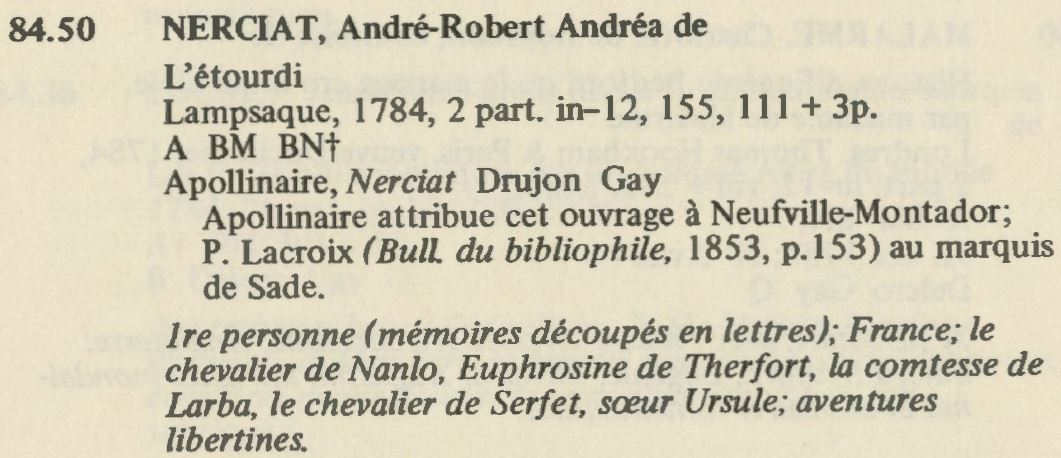
\includegraphics[keepaspectratio]{img_06/etourdi.JPG}}

}

\caption{\label{fig-etourdi}Bibliographischer Eintrag 84.50 zu
\emph{L'étourdi} (Martin / Mylne / Frautschi 1977: 272).}

\end{figure}%

Da die beiden Quellen verschiedene Aussagen hinsichtlich der Autorschaft
des Romans enthalten, eignet sich das Werk gut als Fallbeispiel für eine
stilometrische Analyse hinsichtlich der Frage der Autorschaft. Da die
Frage der Autorschaft nicht völlig offen ist, sondern es eine begrenzte
Zahl von möglichen Kandidaten gibt, können wir im hier skizzierten
Forschungsdesign in Anlehnung an Burrows (2002) von einem `closed
game'\footnote{cf.~Burrows (2002): ``The closed games take two forms.
  Where only two or three writers are eligible candidates for the
  authorship of a particular text and where that text is of a sufficient
  length, we are now well equipped to form strong inferences about their
  rival claims. The classic study of this kind is Mosteller and Wallace
  (1964). Holmes (2001) offers an excellent recent specimen. Where the
  real question is whether or not a particular writer (and no other) is
  the author, we are equally well equipped to test his or her claims.''}
sprechen.

\subsection{Korpuszusammensetzung und
Textgrundlage}\label{korpuszusammensetzung-und-textgrundlage}

In einem ersten Analyseschritt wurde ein Subkorpus zu roman18 erstellt,
welches pro Autor mindestens drei Werke enthält. Dazu wurde eine
SPARQL-Abfrage verfasst, die das Volltextkorpus roman18 nach diesem
Kriterium filtert (Figure~\ref{fig-subcorpus}).

\begin{figure}

\centering{

\pandocbounded{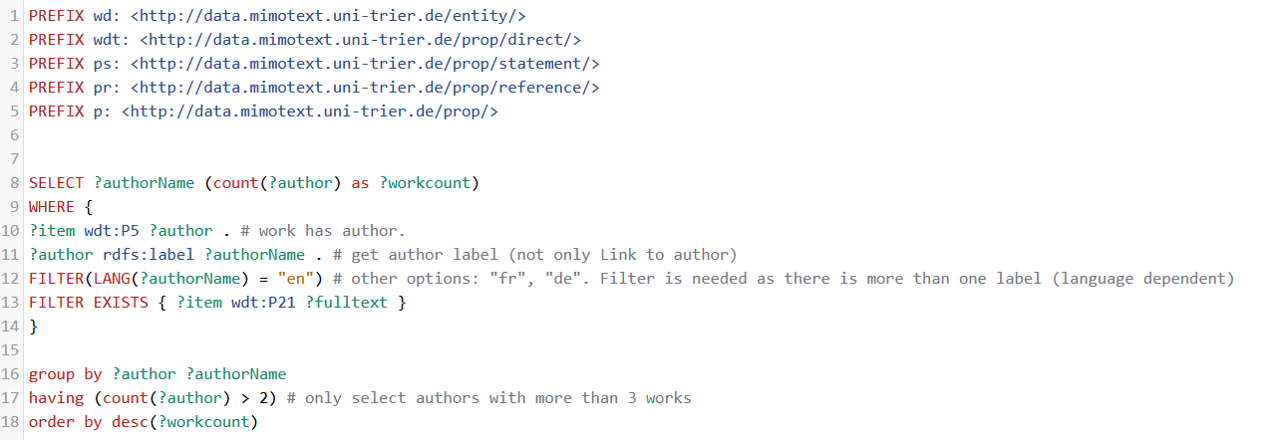
\includegraphics[keepaspectratio]{sparql_3_works_per_authors_subcorpus.png}}

}

\caption{\label{fig-subcorpus}SPARQL-Query: Files mit Volltext-URL und
mindestens drei Werken pro Autor:in,
\url{https://tinyurl.com/232rx7wb}.}

\end{figure}%

Das so gefilterte Korpus ergab folgende Autor:innen mit ihrer Anzahl an
Werken:

\begin{longtable}[]{@{}
  >{\raggedright\arraybackslash}p{(\linewidth - 2\tabcolsep) * \real{0.5000}}
  >{\raggedright\arraybackslash}p{(\linewidth - 2\tabcolsep) * \real{0.5000}}@{}}
\toprule\noalign{}
\begin{minipage}[b]{\linewidth}\raggedright
Autor:in
\end{minipage} & \begin{minipage}[b]{\linewidth}\raggedright
Anzahl
\end{minipage} \\
\midrule\noalign{}
\endhead
\bottomrule\noalign{}
\endlastfoot
ARNAUD, François-Thomas-Marie de Baculard d' & 15 \\
VOLTAIRE, François-Marie Arouet de & 14 \\
CHARRIÈRE, Isabelle-Agnès-Elisabeth van Tuyll van Serooskerken van
Zuylen, dame de & 8 \\
DIDEROT, Denis & 7 \\
RICCOBONI, Marie-Jeanne Laboras de Mézières, madame & 7 \\
SADE, Donatien-Alphonse-François, marquis de & 6 \\
NERCIAT, André-Robert Andréa de & 5 \\
RÉTIF DE LA BRETONNE, Nicolas-Edme & 5 \\
DUCRAY-DUMINIL, François-Guillaume & 4 \\
GENLIS, Stéphanie-Félicité Ducrest de Saint-Aubin, marquise de Sillery,
comtesse de & 4 \\
MARMONTEL, Jean-François & 4 \\
PIGAULT-LEBRUN, Charles-Antoine-Guillaume Pigault de l'Epinay, dit &
4 \\
ROUSSEAU, Jean-Jacques & 4 \\
CAZOTTE, Jacques & 3 \\
CRÉBILLON, Claude-Prosper Jolyot de & 3 \\
DUVERNET, abbé Théophile-Imarigeon & 3 \\
FLORIAN, Jean-Pierre Claris de & 3 \\
LEPRINCE DE BEAUMONT, madame Marie & 3 \\
LOAISEL DE TRÉOGATE, Joseph-Marie & 3 \\
MERCIER, Louis-Sébastien & 3 \\
\end{longtable}

Es ist wichtig, pro Autor:in mehrere Werke im Untersuchungskorpus und
damit genug textuelles Untersuchungsmaterial zu haben, um eine
erfolgreiche stilometrische Analyse durchzuführen (cf. Eder 2015). Die
verwendeten Texte sind zuvor normalisiert und modernisiert worden,
Phänomene wie historische Verbformen im Französisch des 18. Jahrhunderts
oder Verwendung von Schaft-S wurden so ersetzt.\footnote{Eine
  detaillierte Beschreibung dazu in Kapitel 2: Korpusaufbau.}

In einem ersten Analyseschritt wurden die Werke als Plaintext im Tool
Stylo (Eder / Rybicki / Kestemont 2016) in R mit folgenden Einstellungen
analysiert: Wurzburg distance, 2000 MFW. Bevor wir die ersten Ergebnisse
anschauen und analysieren sei hier in Erinnerung gerufen, dass die
stilometrische Analyse nicht nur Hinweise auf die Autorschaft geben
kann, sondern dass ebenfalls Gattungssignale, der Publikationszeitrahmen
oder thematische Nähe ein Einflussfaktor für eine große Nähe zwischen
zwei Werken sein kann.

\begin{figure}

\centering{

\pandocbounded{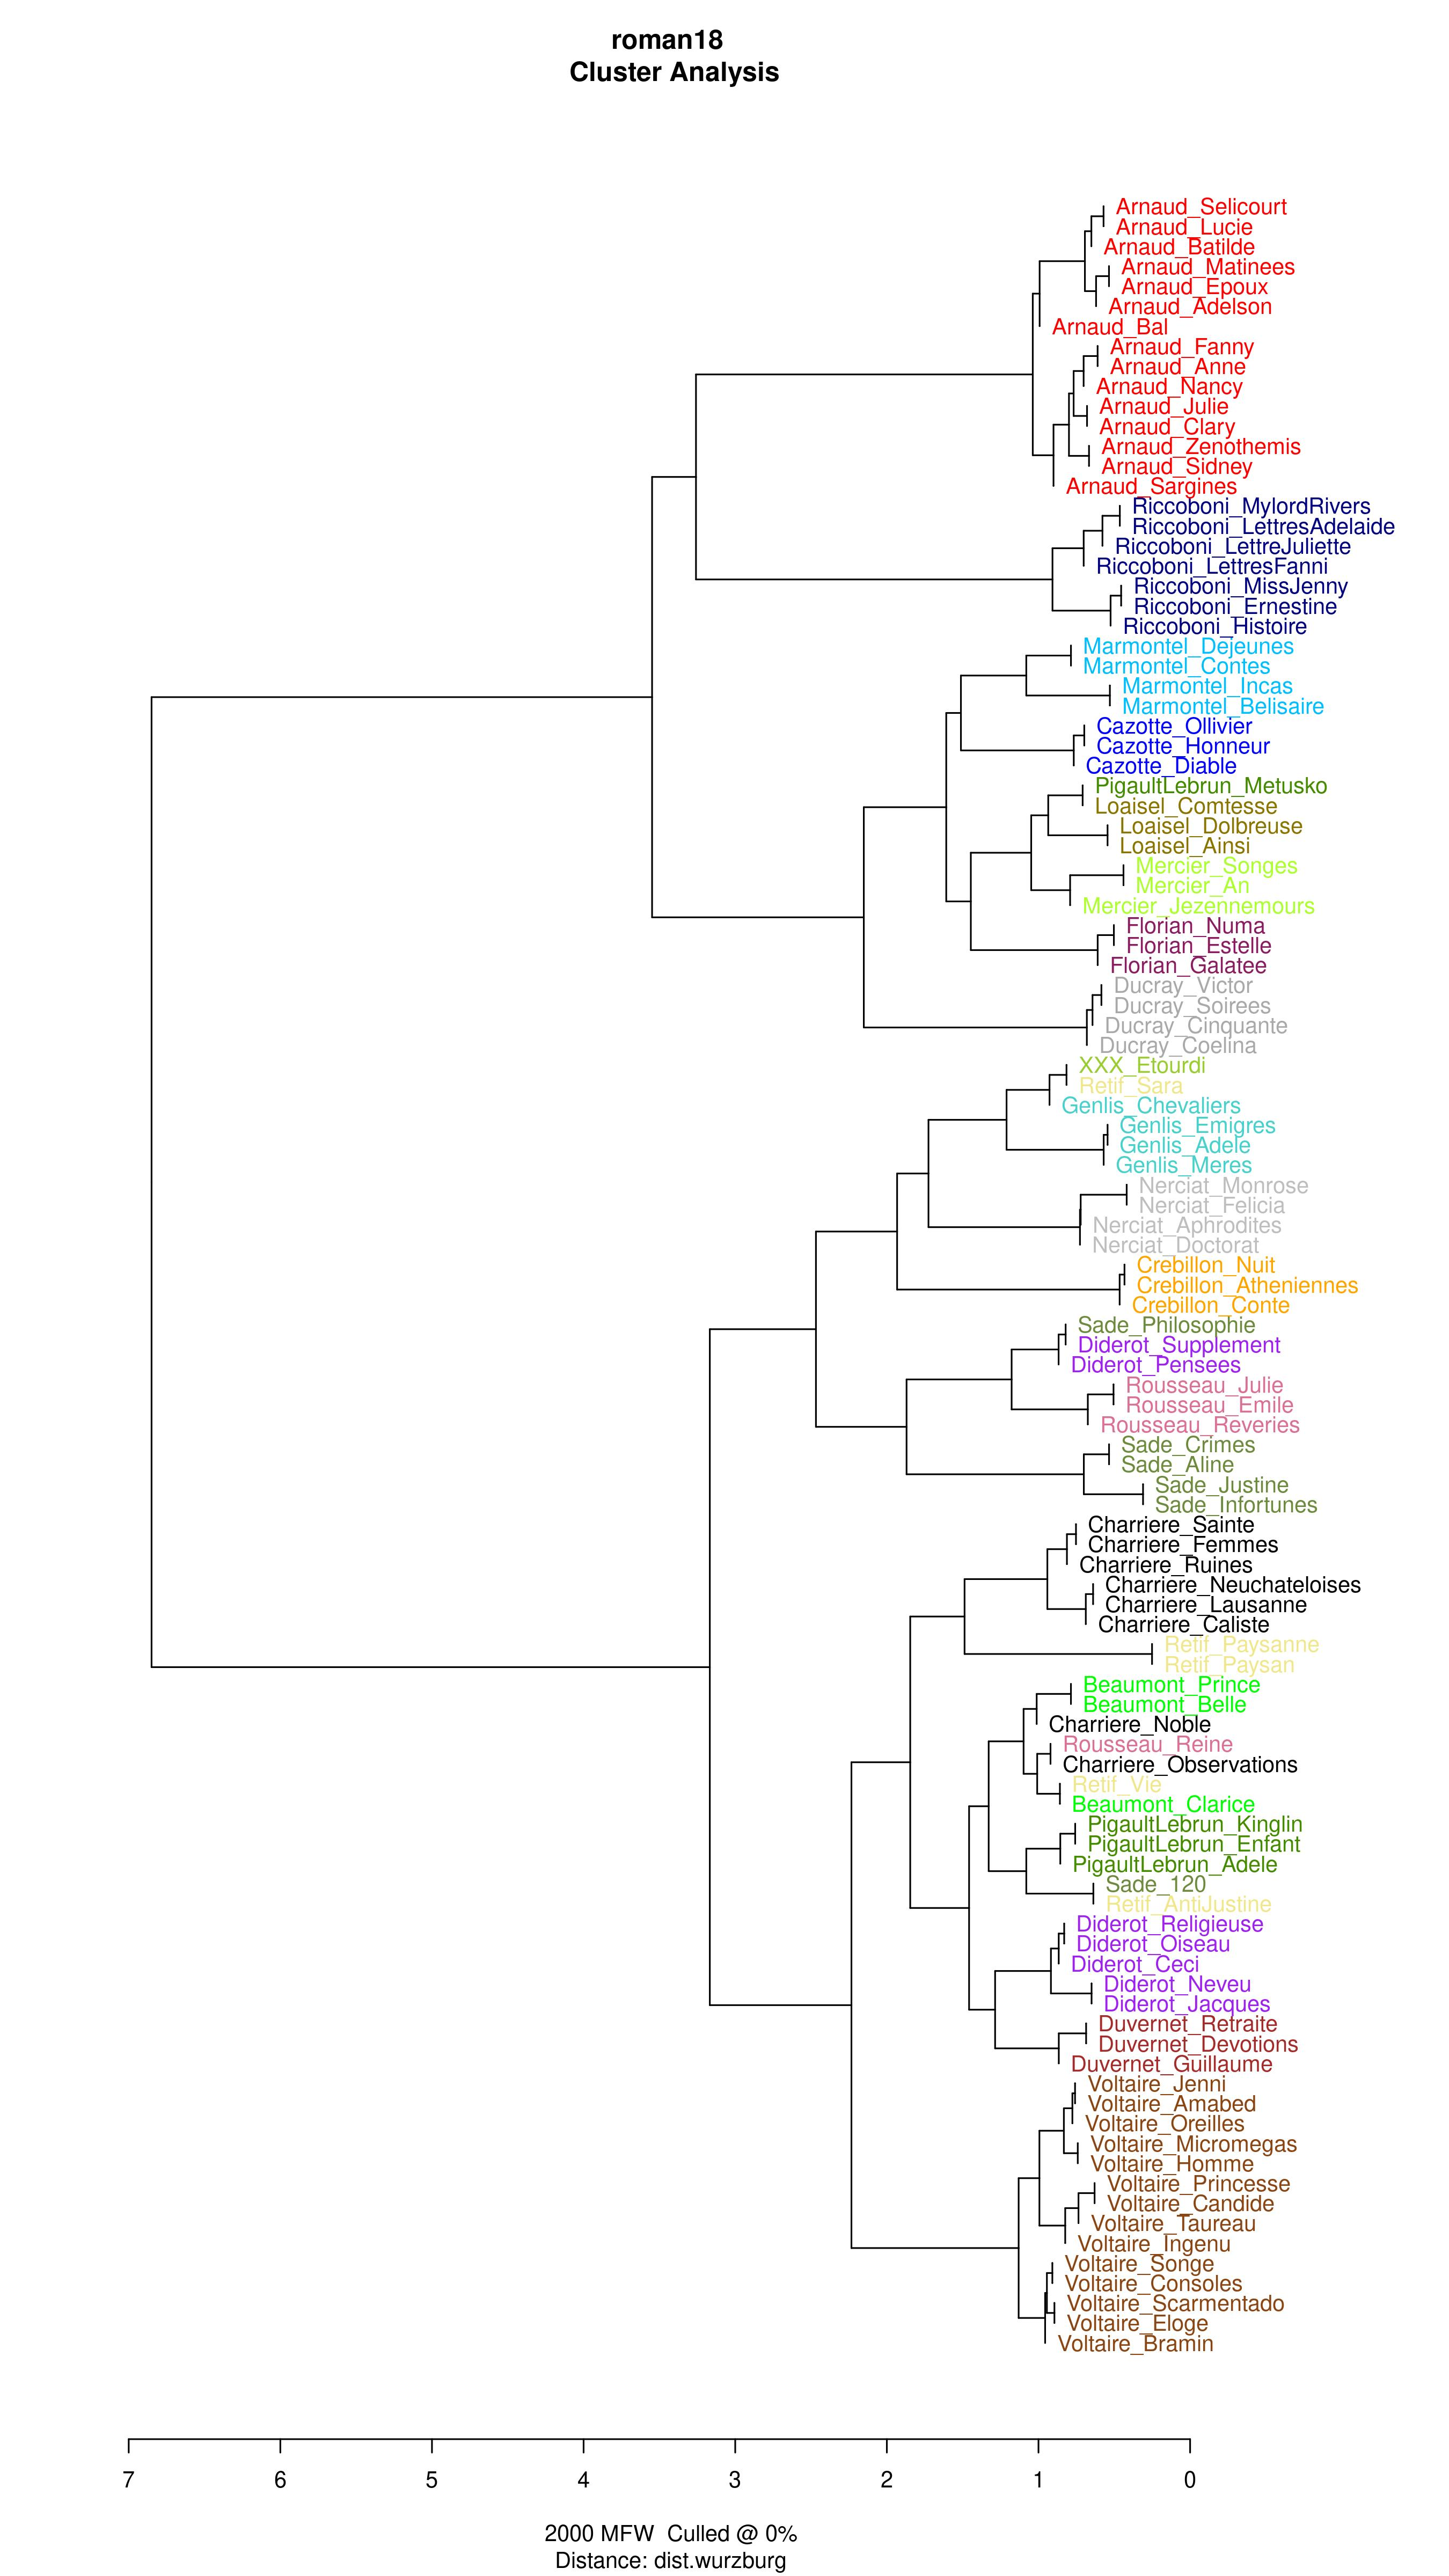
\includegraphics[keepaspectratio]{img_06/wurzburg_distance_2000MFW.jpg}}

}

\caption{\label{fig-wurzburg-distance}Stilometrische Untersuchung von
roman18 mit stylo, Wurzburg distance, 2000 MFW.}

\end{figure}%

Hinsichtlich der genannten potentiellen Autoren (Nerciat, Sade) lässt
sich im von Stylo verwendeten Hierarchical Ward Clustering im ersten
Durchlauf kein eindeutiges Ergebnis erkennen. Der untersuchte Roman
clustert weder eng mit den Romanen von Sade, noch mit Nerciats Werken
Figure~\ref{fig-wurzburg-distance}. Je näher die Werke an einem Ast des
Dendrograms liegen, desto näher ist auch ihre stilometrische
Ähnlichkeit.\\
Stylo ermöglicht es, das untersuchte Korpus mit einer Principal
Component Analyse (PCA) zu untersuchen, um jene Elemente darzustellen,
die ausschlaggebende Komponenten der stilometrischen Analyse sind.

\begin{figure}

\centering{

\pandocbounded{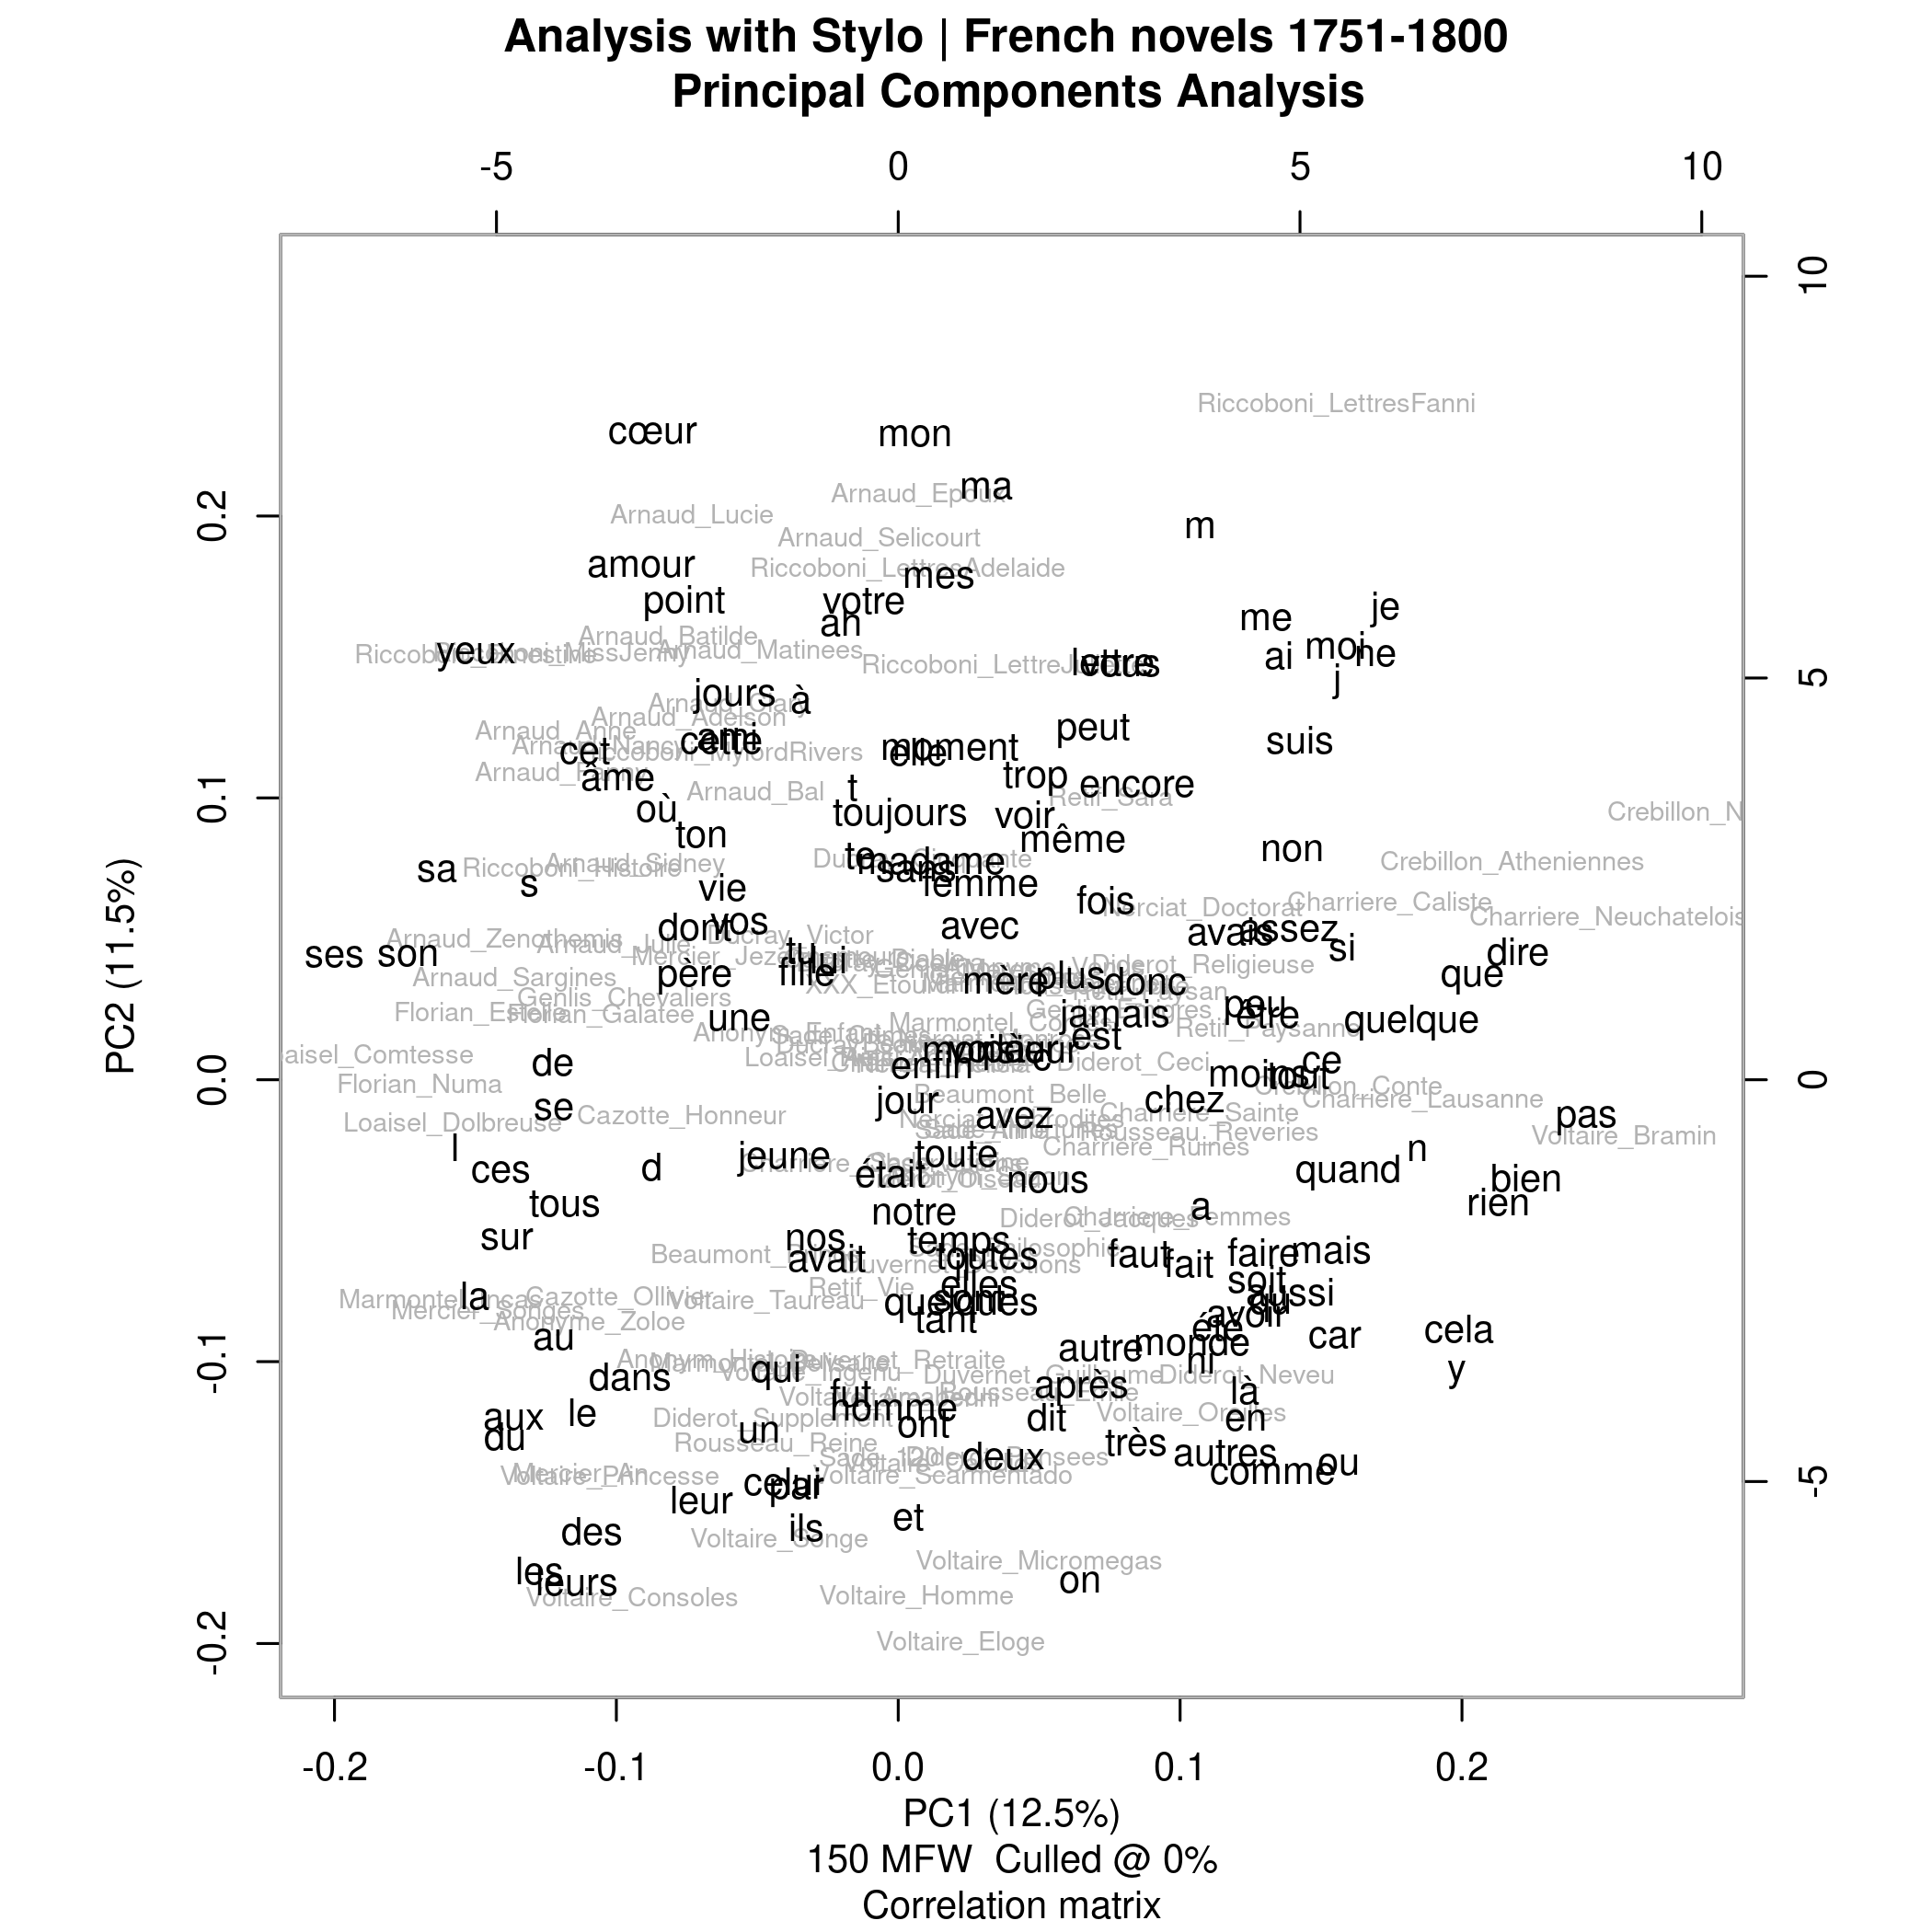
\includegraphics[keepaspectratio]{img_06/150_MFW_pca_loadings.png}}

}

\caption{\label{fig-pca-loadings}PCA(Principal Components Analysis) mit
Loadings}

\end{figure}%

Im oberen Bereich der PCA erkennt man, dass in der Principal Component
Analyse mehrere Werke des gleichen Autors, Baculard d'Arnaud, clustern
(Figure~\ref{fig-pca-loadings}). Die hier visualisierten Loadings sind
`coeur', `mon', `ma' oder `amour'. Es zeigt sich, dass hier einerseits
Funktionswörter ausschlaggebend sind, andererseits ist Baculard d'Arnaud
ein Verfasser einer Vielzahl von Sentimentalromanen. Insofern sind die
hier visualisierten Loadings `coeur' (Herz) oder `amour' (Liebe)
plausibel.\\
Da sich insgesamt im ersten Analyseschritt jedoch keine eindeutige
Zuordnung zu den hypothetischen Autoren im Clustering-Verfahren zeigte,
wurde ein weiterer Durchgang der stilometrischen Analyse durchgeführt.
Einer der potentiellen Autoren, Neufville-Montador, war zunächst nicht
im Romankorpus vertreten. Um zu verifizieren, ob sich hier eine
stilometrische Nähe zeigt, wurden ergänzend erzählende Texte von
Neufville-Montador dem Untersuchungskorpus hinzugefügt.

\subsection{Sollte doch Apollinaire recht
behalten?}\label{sollte-doch-apollinaire-recht-behalten}

Neben Nerciat und Marquis de Sade wird in \emph{L'Enfer de la
Bibliothèque nationale} eine weitere Autorschaftshypothese geäußert:
Neufville-Montador. Könnte es sein, dass doch Apollinaire recht hatte,
als er schrieb:

``Cet ouvrage a été attribué tour à tour et sans beaucoup de raison au
marquis de Sade et au chevalier Andrea de Nerciat. On en a aussi
attribué la paternité, avec plus de vraisemblance, au chevalier de
Neufville-Montador.'' (Apollinaire 1919)

Apollinaire hält demnach Neufville-Montador für den wahrscheinlichsten
Autor. Um dies zu überprüfen, wurde in einem zweiten Schritt das für die
stilometrischen Analysen verwendete Korpus erweitert. Dazu wurde nach
verfügbaren Volltexten des Autors Neufville-Montador recherchiert. Ein
von ihm verfasstes
\href{https://gallica.bnf.fr/services/engine/search/sru?operation=searchRetrieve&version=1.2&collapsing=disabled&query=\%28gallica\%20all\%20\%22neufville-montador\%22\%29\%20and\%20arkPress\%20all\%20\%22cb46635638h_date\%22&rk=64378;0}{\emph{Almanach
nocturne a l'usage du grand m}onde}
\href{https://gallica.bnf.fr/services/engine/search/sru?operation=searchRetrieve&version=1.2&collapsing=disabled&query=\%28gallica\%20all\%20\%22neufville-montador\%22\%29\%20and\%20arkPress\%20all\%20\%22cb46635638h_date\%22&rk=64378;0}{1739-1742},
welches als Faksimile in der digitalen Sammlung der französischen
Nationalbibliothek verfügbar ist, enthält erzählende Passagen, die für
die Analyse verwendet wurden. Außerdem ist ein Roman von
Neufville-Almanach über GoogleBooks verfügbar (Confessions de la Baronne
de ***, 1848). \footnote{Die verwendeten erzählenden Texte von
  Neufville-Montador sind hier einsehbar:
  \url{https://github.com/MiMoText/Stylometric_Analysis/tree/main/corpora/Neufville_Montador}.}
Beide Werke wurden über die bereits beschriebene
Digitalisierungspipeline mithilfe von OCR4all und einem Modell für
französische Drucke des 18. Jahrhunderts erschlossen und als Plaintext
dem bestehenden Korpus hinzugefügt. Wie hat sich mit dem so erweiterten
Datensatz die Analyse verändert?

\begin{figure}

\centering{

\pandocbounded{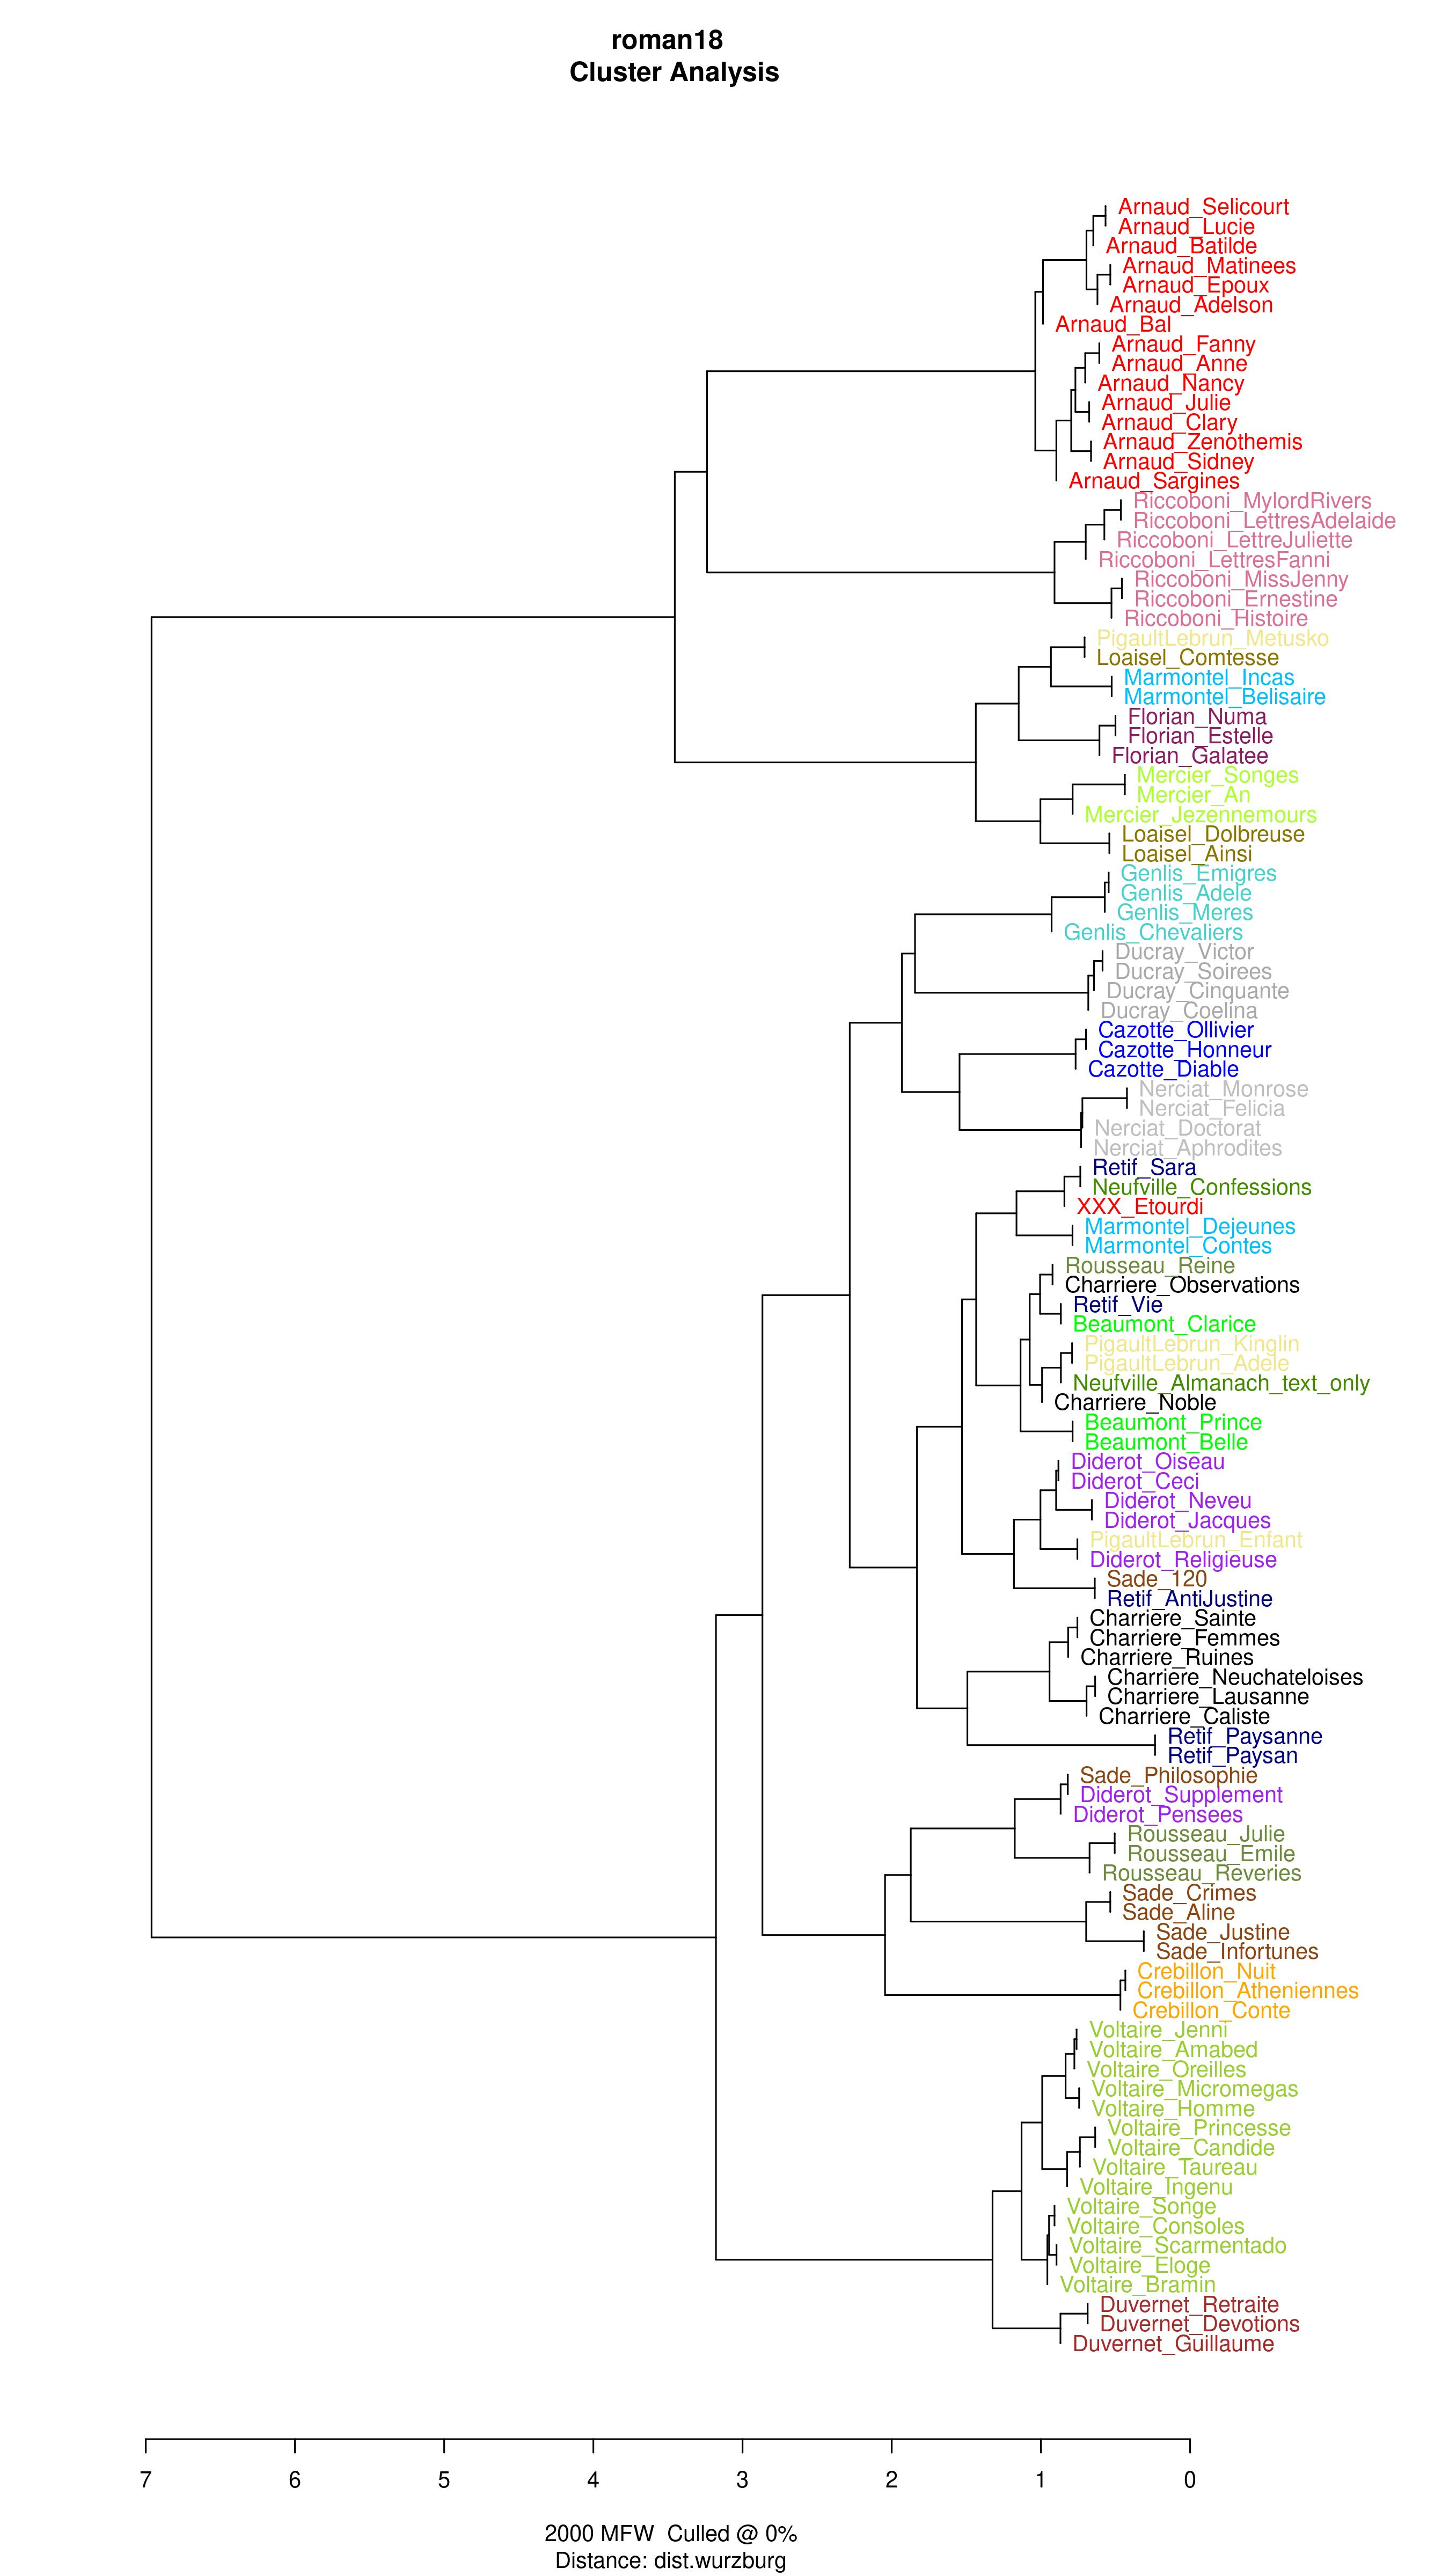
\includegraphics[keepaspectratio]{img_06/with_neufville_montador.jpg}}

}

\caption{\label{fig-with-neufville}Stilometrische Analyse mit
erweiterten Datensatz, 3500 MFW, Wurzburg distance.}

\end{figure}%

Die Abbildung Figure~\ref{fig-with-neufville} der stilometrischen
Analyse mit erweitertem Datensatz zeigt, dass die Werke von Sade
zusammen clustern, die Werke von Nerciat zusammen clustern und das
untersuchte Werk \emph{L'étourdi} von den drei möglichen
Kandidaten-Autoren am nächsten mit Neufville-Montador clustert. Sollte
demnach Apollinaire recht behalten?

Stylo bietet als zusätzliche Möglichkeit der Analyse die Verwendung des
`Bootstrap Consensus Tree' (Figure~\ref{fig-bootstrap-neufville}). Dabei
handelt es sich um eine kreisförmige Visualisierung, die mehrere
Durchläufe der Clusteranalyse mit variierender Anzahl der am häufigsten
vorkommenden Wörter zu einer konsolidierten Ergebnisvisualisierung
zusammenführt. Der Sinn dieser Analyse liegt darin zu überprüfen, wie
stabil das Clustering bei verschiedenen Einstellung der Verwendung der
MFW (most frequent words) ist. Dieser Prozess, auch als `Bootstrap'
bezeichnet, verwebt die individuellen Analysedurchläufe ähnlich dem
Schnüren eines Schuhs (`bootstrapping') und zieht sie am Ende zusammen.
Ähnliche Texte werden hier auf einem Zweig durch Clustering
repräsentiert. Bei der Auswahl des `Consensus Tree' müssen zusätzliche
Parameter im MFW-Setting festgelegt werden, darunter der Start- und
Endpunkt der Analyse (`Minimum' / `Maximum'), sowie die Anzahl der
hinzugefügten Wörter in jeder einzelnen Analyse (`Increment'). In meiner
Analyse habe ich mich für einen Startwert von 2000, ein Inkrement von
100 Wörtern und ein Maximum von 4000 entschieden. Bei dieser Höhe der
verwendeten meist frequenten Wörter (2000+) ist von einer Mischung aus
Funktions- und Inhaltswörtern auszugehen.

\begin{figure}

\centering{

\pandocbounded{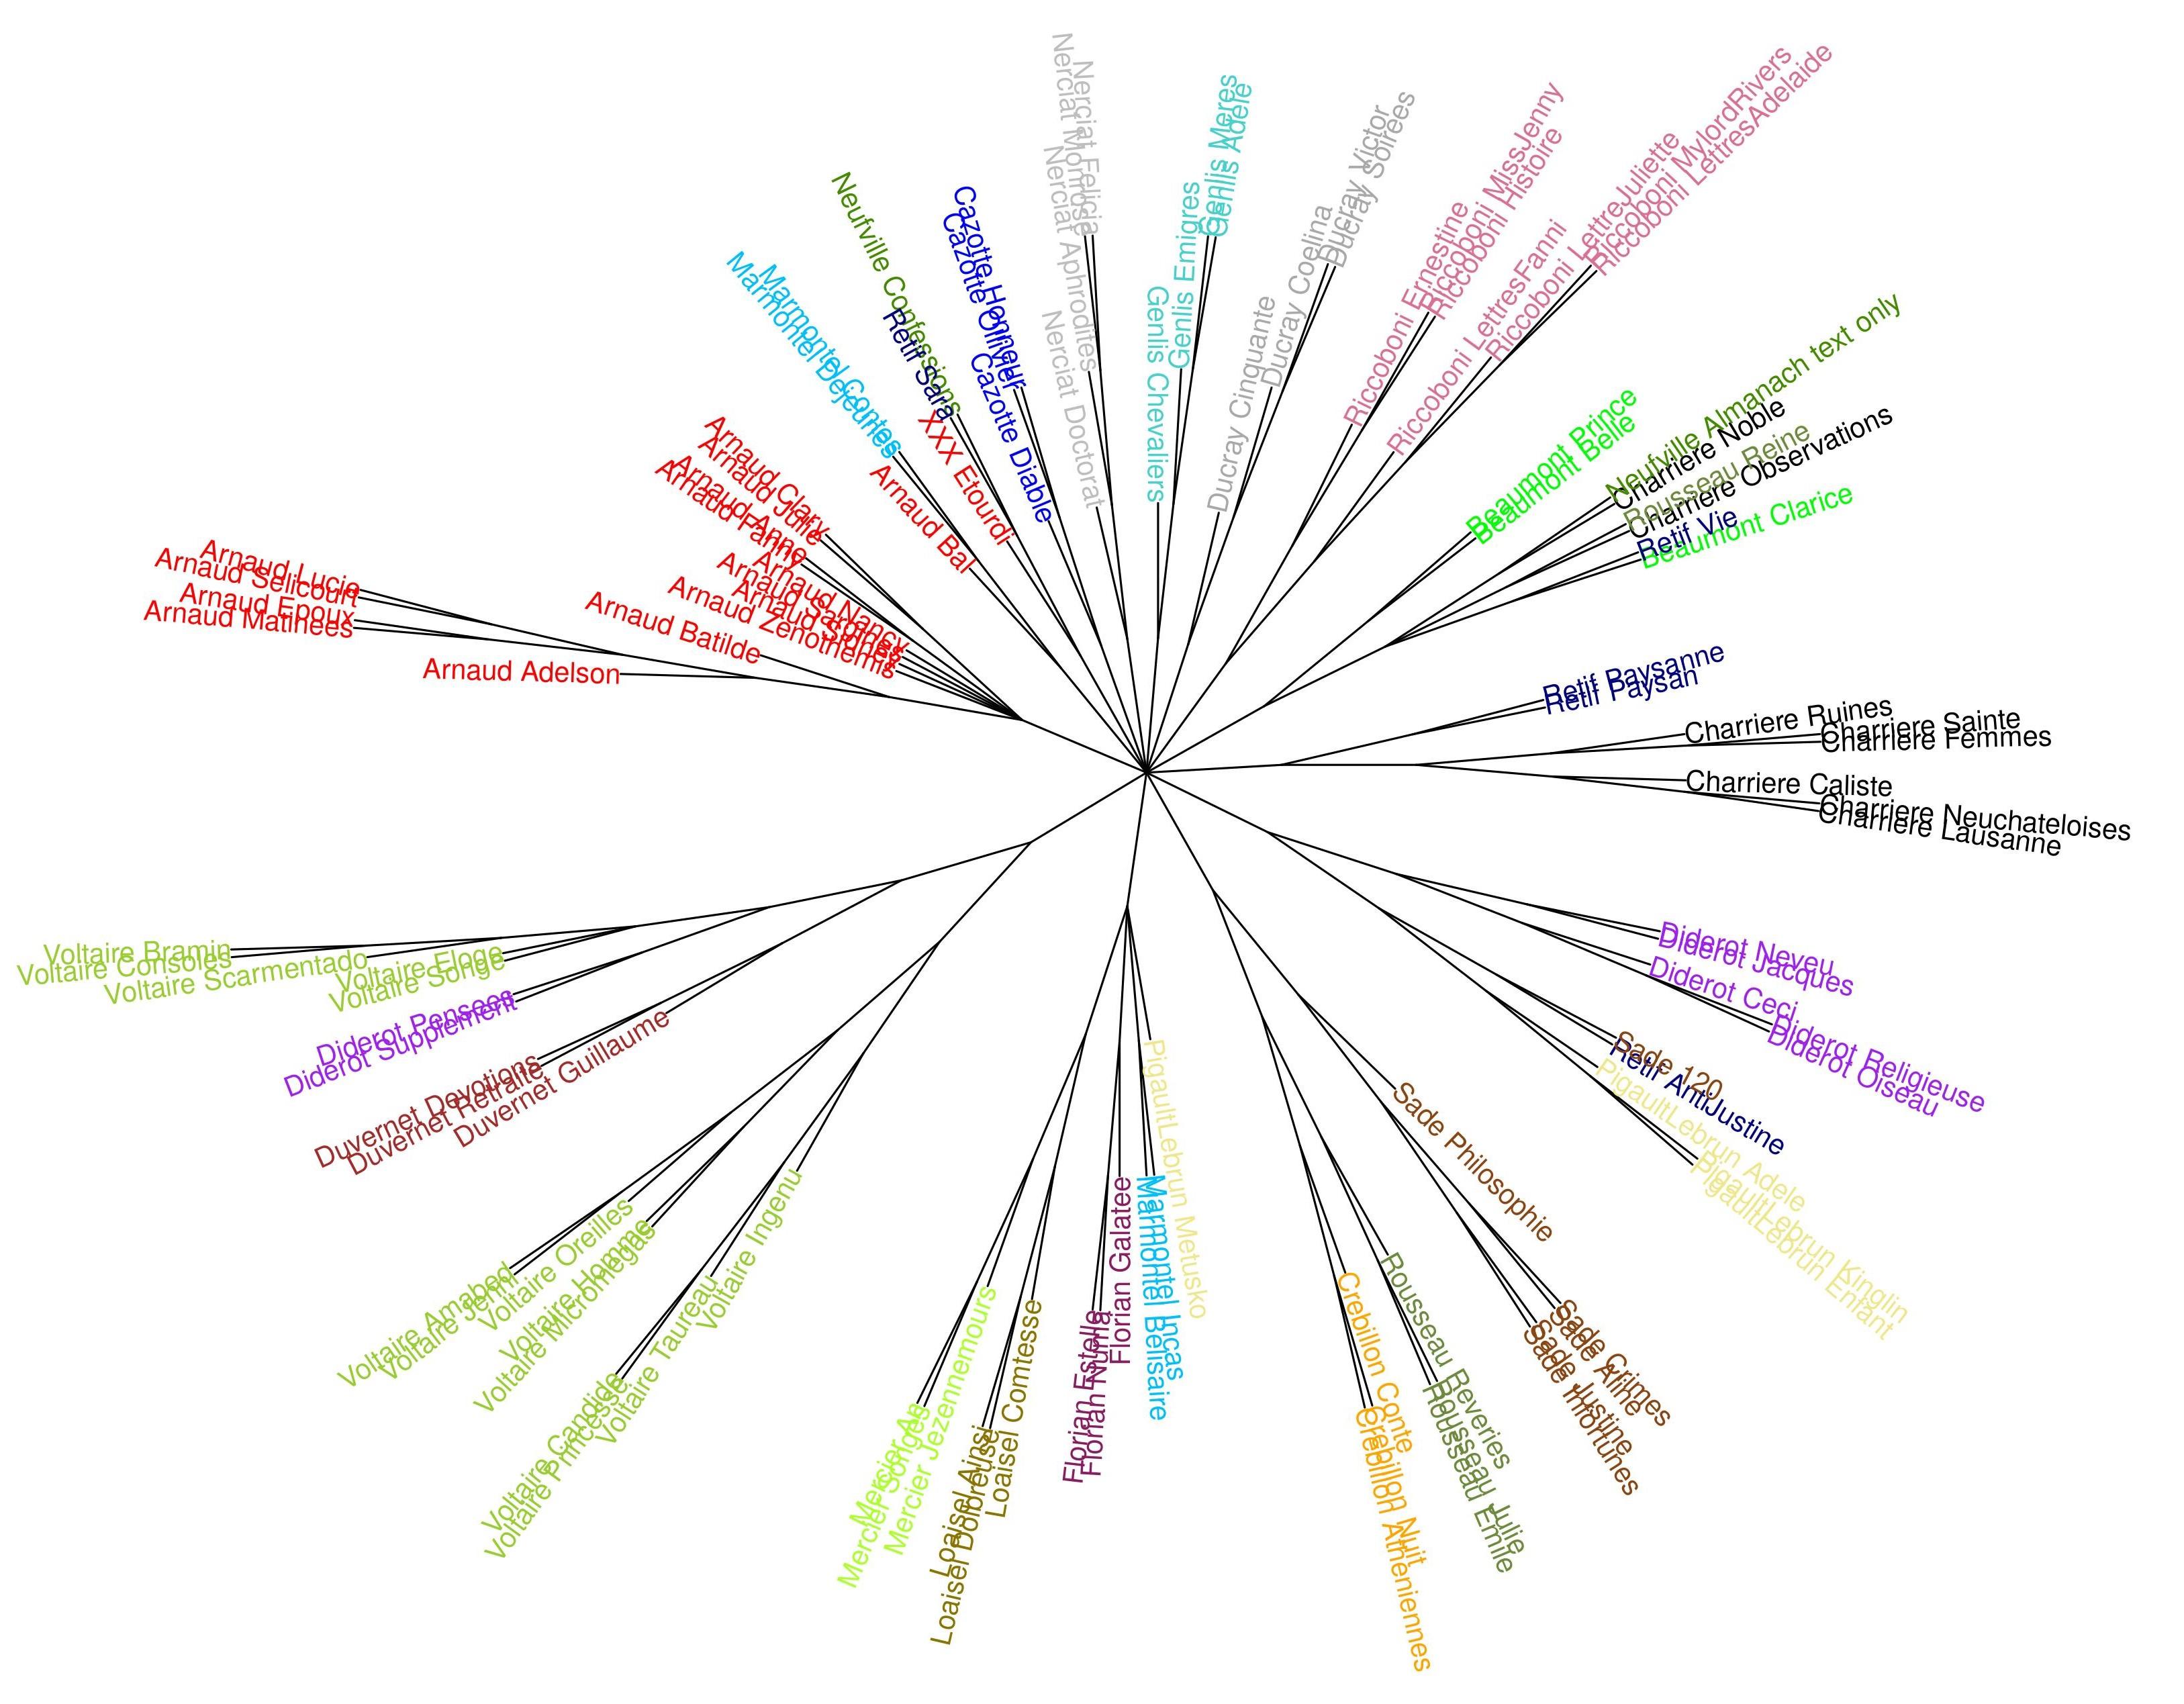
\includegraphics[keepaspectratio]{img_06/bootstrap_consensus_tree_with_neufville.jpg}}

}

\caption{\label{fig-bootstrap-neufville}Bootstrap consensus tree,
Wurzburg distance, 2000-4000 MFW.}

\end{figure}%

Das schrittweise Erhöhen des Parameter der am häufigsten vorkommenden
Wörter (MFW) im Bootstrap Consensus Tree zeigt, dass die Nähe des Textes
\emph{L'Étourdi} zu den verwendeten Texten mit Autorschaft von
Neufville-Montador relativ stabil ist
(Figure~\ref{fig-bootstrap-neufville}). Unter der Annahme, dass entweder
Marquis de Sade, Andréa de Nerciat oder Neufville-Montador der Autor von
\emph{L'Étourdi} ist, können wir anhand der Ergebnisse dieser
stilometrischen Untersuchung mit dem Tool Stylo in R feststellen, dass
Neufville-Montador im hier untersuchten Setting aus der Kandidatenliste
als der wahrscheinlichste Autor des Romans gelten kann.

\subsection{Überraschende Erkenntnis: Dendrogram und numerische
Distanzwerte legen verschiedene Hypothesen
nahe}\label{uxfcberraschende-erkenntnis-dendrogram-und-numerische-distanzwerte-legen-verschiedene-hypothesen-nahe}

Die bisherige Analyse stützte sich wie eine Vielzahl an stilometrischen
Studien, die in den Digital Humanities durchgeführt werden auf die
Erkenntnis aus der Visualisierung der Dendrogramme oder Bootstrap-Trees.
Eine Nähe auf einem Ast des durch Clustering generierten Trees ließ auf
eine Nähe der Werke und somit Autorschaften schließen. Diese Annahme ist
zwar grundsätzlich nicht als falsch anzusehen und ein Großteil der
stilometrischen Studien in den Digital Humanities geht hier ähnlich vor,
jedoch zeigte sich überraschenderweise im hier untersuchten Fall, dass
Dendrogram und numerische Werte unterschiedliche Autorschaftshypothesen
nahe legen. Während das Hierarchical Wards Clustering
Neufville-Montadors Werke auf dem nächsten Ast zu \emph{L'étourdi}
verortete, zeigen die rohen numerischen Werte ein anderes Bild: Hier
liegt Nerciats Werk \emph{Félicia} am nächsten zu \emph{L'étourdi} und
legt somit eine Autorschaft Nerciats nahe.

\begin{figure}

\centering{

\pandocbounded{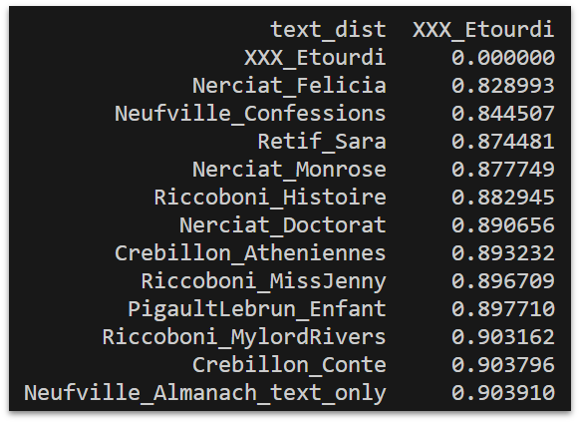
\includegraphics[keepaspectratio]{img_06/stylometry_numerical.png}}

}

\caption{\label{fig-numerical}Distance table, 3500 MFW, Wurzburg
distance.}

\end{figure}%

Im Clustering-Prozess ist jeweils von einem gewissen Informationsverlust
auszugehen, sodass hier die numerischen Werte die verlässlichere Quelle
darstellen.\footnote{Die anhand des Fallbeispiels festgestellte
  Diskrepanz wurde anlässlich des Workshops \emph{Potentials and Limits
  of Stylometry for Early Modern Text in Romance Languages} am 11.
  Oktober 2023 am Trier Center for Digital Humanities im Anschluss an
  den Vortrag ``Decoding Literary Signatures: Stylometric Insights into
  Authorship Attribution in 18th Century French Novels'' diskutiert. An
  dieser Stelle Dank an Artjoms Šeja (Institute of Polish Language,
  Polish Academy of Sciences) und Christof Schöch (Trier Center for
  Digital Humanities ) für Anregung und Hinweise.} Diese bilden daher
auch die Grundlage der im Knowledge Graphen importierten Resource
Description Framework (RDF) Triples zur stilometrischen Analyse der
Romane.\\
Eine qualitative Bewertung des Romans und der potentiell ähnlichen Werke
anhand der bei Lektüre festgestellten stilistischen Merkmale wären neben
der stilometrischen Analyse ein weiterer ergänzender Schritt, der hier
jedoch nicht Gegenstand der Untersuchung ist. \footnote{Gleichwohl
  finden sich in der Fachliteratur weitere Hinweise, beispielsweise im
  Vorwort einer deutschen Übersetzung: ``Dieser galante Roman, der die
  Jugend eines solchen Lebemannes schildert, zeichnet ein treffendes
  Sittengemälde der französischen Gesellschaft des Ancien Régime
  unmittelbar vor der Revolution. Wenngleich dieser Roman auch anonym
  erschienen ist, dürfte A. de Nerciat der Verfasser sein. An dieser
  Zuschreibung, die uns durch die Tradition überliefert ist, haben wir
  keinen Grund zu zweifeln, weil auch stilistische und sprachliche
  Gründe dafür sprechen.'' (Werner 2014: pp.4).}

In einigen Beispielen an SPARQL-Abfragen sei nun illustriert, wie sich
diese Statements abfragen lassen und welche Schlüsse sich daraus ziehen
lassen.

\section{Abfrage der stilometrischen Analyse in
SPARQL}\label{abfrage-der-stilometrischen-analyse-in-sparql}

Die Ergebnisse der hier beschriebenen Analyse sind hinsichtlich der
numerischen Werte der stilometrischen Ähnlichkeit im Knowledge Graphen
als Statements importiert. Dies ermöglicht es, über entsprechende
SPARQL-Abfragen bezogen auf Einzelwerke oder Autoren nach den - laut
stilometrischer Analyse - ähnlichsten Werken zu fragen. Ich gehe daher
in SPARQL-Abfagen der Frage nach, welche Gemeinsamkeiten Werke haben,
die sich stilometrisch nah sind: Teilen Sie die Erzählform, Autorschaft
oder Tonalität?\\
Zunächst eine Abfrage, die verdeutlicht, welche Werke stilometrisch nah
zu Rousseaus Werken sind.

\section{\texorpdfstring{\href{http://tinyurl.com/ylafpk9d}{Rousseaus
Werke im Graphen und Werke, die jenen stilometrisch ``nah''
sind}}{Rousseaus Werke im Graphen und Werke, die jenen stilometrisch ``nah'' sind}}\label{rousseaus-werke-im-graphen-und-werke-die-jenen-stilometrisch-nah-sind}

Man sieht in den Ergebnissen der Abfrage, dass die nächsten Werke häufig
diejenigen des untersuchten Autors (hier: Rousseau) sind. Zu seiner
fabel-/märchenhaften Erzählung
\href{https://data.mimotext.uni-trier.de/wiki/Item:Q1379}{\emph{La reine
Fantasque}} (1758) hingegen sieht man in der Listung der ähnlichsten
Werke auch Werke, die ebenfalls Märchen sind, beispielsweise
\href{https://data.mimotext.uni-trier.de/wiki/Item:Q1013}{\emph{Ah! quel
conte!}} (1754) von Crébillon. Gemeinsamkeiten dieser beiden Werke sind
unter anderem ihre Erzählform (``3e personne''), ihr Handlungsort
(``cadre fantaisiste``), auch einige aus Topic Modeling hervorgegangene
Themenwerte (``monarchie''\footnote{\url{https://data.mimotext.uni-trier.de/wiki/File:Wordle_topic_modeling_2023_topic_039_monarchie.png}.})
oder ähnliche Hauptfiguren (``la fée Discrette'' / ``la fée
Toutou-rien'').\\
In diesem Beispiel zeigt sich, dass das Gattungssignal je nach
Vergleichskorpus durchaus das Autorschaftssignal überlagern kann.

Wir haben im Knowledge Graphen über SPARQL-Abfragen die Möglichkeit uns
anzusehen, welche Gemeinsamkeiten Werke haben, die in einer
stilometrischen Analyse unter den nächst ähnlichen Werken sind: Haben
Sie den gleichen Autor oder die gleiche Autorin? Teilen Sie die
narrative Form? Stimmt ihre Tonalität überein?

\section{\texorpdfstring{\href{https://tinyurl.com/24q38l55}{Welche
Gemeinsamkeiten haben Werke, die sich basierend auf einer
stilometrischen Analyse ähnlich sind: Autor, Tonalität, narrative
Form?}}{Welche Gemeinsamkeiten haben Werke, die sich basierend auf einer stilometrischen Analyse ähnlich sind: Autor, Tonalität, narrative Form?}}\label{welche-gemeinsamkeiten-haben-werke-die-sich-basierend-auf-einer-stilometrischen-analyse-uxe4hnlich-sind-autor-tonalituxe4t-narrative-form}

Für insgesamt \textbf{657 Statements} zu französischen Romanen
1751-1800, die über eine stilometrische Nähe\footnote{Stilometrisch nah
  im Graphen sind Werke, die unter den nächst ähnlichen Werken basierend
  auf der beschriebenen stilometrischen Analyse sind. Der Cut-Off liegt
  im Knowledge Graphen bei den fünf ähnlichsten Werken.} und Angaben zu
Tonalität, narrativer Form und Autor:in verfügen, ergibt sich dabei
folgendes Bild: Bei 369 Statements zu stilometrischer Nähe stimmt die
narrative Form überein. Bei 382 Statements stimmt der Autor oder die
Autorin überein. Bei 157 Statements stimmt die Tonalität der Werke
überein, also haben die Werke jeweils den gleichen Wert wie
beispielsweise ``satire'' oder ``mélancolie''.

Diese Varianten der SPARQL-Abfragen legen nahe, dass von den gemeinsamen
Features im Graphen das Autorschaftssignal am häufigsten zu einer
stilometrischen Nähe zweier Werke führt, gefolgt von der narrativen Form
(als Beispiel: `epistolary').

\section{Modellierung des Ergebnisses in
Wikibase}\label{modellierung-des-ergebnisses-in-wikibase}

Können wir im Hinblick auf das diskutierte Fallbeispiel der
Autorschaftsfrage von \emph{L'Étourdi} mit Sicherheit sagen, dass,
basierend auf den numerischen Ergebnissen der vorgestellten
stilometrischen Analyse, Nerciat der Autor war? Dies ist in dieser
Eindeutigkeit sicher nicht möglich, da die stilometrische Analyse
einerseits vom Vergleichskorpus und andererseits von weiteren
Einflussfaktoren abhängen kann (Schöch 2017, pp.~296). Schon Burrows
spricht in seiner wegweisenden Studie von ``likely authorship'' (Burrows
2002). So hat neben dem Autorschaftssignal auch die thematische Nähe
oder ähnliche Gattung einen Einfluss darauf, ob sich Werke in der
Analyse nah sind. Es wäre auch möglich, dass eine weitere historische
Quelle entdeckt wird, die einen noch nicht im Korpus vertretenen Autor
als wahrscheinlichsten Autor annimmt und dessen Werke in der hier
vorgestellten Analyse nicht mit berücksichtigt sind, dessen Werke jedoch
noch näher an \emph{L´Étourdi} liegen. Für die berücksichtigten Quellen
und das vorgestellte untersuchte Korpus können wir jedoch sagen, dass
unter den drei möglichen Autoren die wahrscheinlichste Variante laut
stilometrischer Analyse mit den beschriebenen Parametereinstellungen
Nerciat darstellt.

Wie lässt sich nun dieses Ergebnis im Knowledge Graphen modellieren?
Müssen wir uns hinsichtlich der Werk-Person Relation `author of' im
Graphen für einen eindeutigen Wert entscheiden? In der verwendeten
Infrastruktur (Wikibase) ist es durchaus möglich, alle drei Varianten
als Statements aufzunehmen und über einen weiteren Qualifier (`rank')
eine Abstufung der Wahrscheinlichkeiten vorzunehmen. Wikibase bietet die
Möglichkeit Statements mit einem `rank' zu versehen:
\texttt{wikibase:PreferredRank}, \texttt{wikibase:NormalRank} und
\texttt{wikibase:DeprecatedRank} sind die Abstufungen, die hier gewählt
werden können Figure~\ref{fig-ranks}.\footnote{``Another type of
  built-in annotation on statements is the \emph{statement rank}, which
  can be \emph{normal} (default), \emph{preferred}, or
  \emph{deprecated}. Ranks are a simple filtering mechanism when there
  are many statements for one property''. (Malyshev et al. 2018:
  pp.379).} Dies bietet die Möglichkeit, konfligierende Aussagen im
Graphen zu integrieren. Die Ergebnisse der stilometrischen Analyse
können so in Wikibase abgebildet werden:

NERCIAT, André-Robert Andréa de - \textgreater{} preferred rank\\
NEUFVILLE DE BRUNABOIS-MONTADOR, chevalier Jean-Florent-Joseph de
-\textgreater{} normal rank\\
SADE, Donatien-Alphonse-François, marquis de -\textgreater{} deprecated
rank

\begin{figure}

\centering{

\pandocbounded{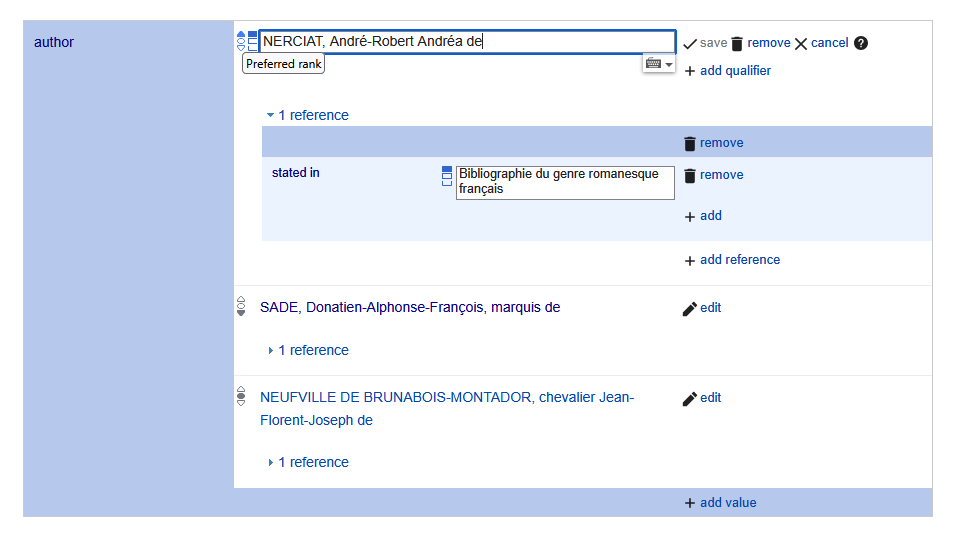
\includegraphics[keepaspectratio]{img_06/ranks_wikibase.png}}

}

\caption{\label{fig-ranks}Preferred rank, normal rank und deprecated
rank in Wikibase (MiMoTextBase)}

\end{figure}%

Sollten spätere Analysen oder neue Quellen eine veränderte Sachlage
ergeben, können die Ranks der möglichen Werte auch wieder neu justiert
werden. Werden in SPARQL-Abfragen keine `ranks' spezifiziert, so wird
üblicherweise der Wert, der mit `preferred rank' gekennzeichnet ist, als
Ergebnis ausgegeben.\footnote{SPARQL-Abfrage: Wer ist der Autor von
  L'Étourdi? \url{http://tinyurl.com/yvmpfk6q}.}\\
Zusätzlich zu dieser möglichen Abstufung der Statements wurden für die
hier beschriebene stilometrische Analyse in den Graphen die numerischen
Werte, die aus der Analyse hervorgegangen sind, als Statements
importiert.\footnote{Die entsprechende Property heißt P49 (``stylometric
  based similarity''),
  https://data.mimotext.uni-trier.de/wiki/Property:P49.} Im Gegensatz
zum Clustering Dendrogram erlauben die rohen numerischen Werte im
Knowledge Graphen präzisere Aussagen hinsichtlich der stilometrischen
Nähe zweier Werke (cf. Schöch 2023).

\section{Zusammenfassung}\label{zusammenfassung}

Im vorliegenden Kapitel ließ sich zeigen, wie eine umstrittene
Autorschaft eines französischen Romans des 18. Jahrhunderts mithilfe der
Computational Literary Studies Methode Stilometrie zwar nicht
abschließend geklärt werden kann, jedoch aus einer Auswahl an möglichen
Kandidaten (`closed game') der wahrscheinlichste Kandidat
herauskristallisiert werden konnte. Neben dem klassischen Hierarchical
Wards Clustering (Ward 1963) wurde zusätzlich ein Bootstrapping
angewandt, um zu überprüfen, wie stabil die stilometrische Nähe von
Werken bei unterschiedlichen Parametereinstellungen (Anzahl der
verwendeten most frequent words) ist. Die numerischen Werte der
Ähnlichkeiten wichen jedoch von den ``next neighbours'' im
Clustering-Verfahren ab und wurden als verlässlicherer Wert im Graphen
importiert.\\
Aus den möglichen Autor-Kandidaten - hervorgegangen aus historischen
Quellen - wurden die Kandidaten Sade, Nerciat und Neufville-Montador
identifiziert. Aus den drei möglichen Kandidaten geht in der hier
beschriebenen Analyse als wahrscheinlichste Variante eine Autorschaft
Nerciats hervor. Die Methode Stilometrie kann so datenbasiert zu einer
Literaturgeschichte des französischen Romans des 18. Jahrhunderts
hinsichtlich von offenen Fragen der Autorschaft beitragen.\\
Die Modellierung in Wikibase zeigt, dass im Knowledge Graphen
konfligierende Aussagen nebeneinander stehend importiert werden können.
Die Nutzung von Rängen (`ranks') ermöglicht über die Qualifizierung von
Statements eine Abstufung der Plausibilität der möglichen
Autorschafts-Varianten.

\section{Bibliographie}\label{bibliographie}

\phantomsection\label{refs}
\begin{CSLReferences}{1}{0}
\bibitem[\citeproctext]{ref-apollinaire_lenfer_1919}
\textbf{Apollinaire, Guillaume} (1919):
\emph{\href{https://fr.wikisource.org/wiki/Livre:Apollinaire_-_L\%E2\%80\%99Enfer_de_la_Biblioth\%C3\%A8que_nationale.djvu}{L'{Enfer}
de la {Bibliothèque} nationale}}. Bibliothèque des curieux.

\bibitem[\citeproctext]{ref-burrows_delta_2002}
\textbf{Burrows, John} (2002): "{„{Delta}``}: a {Measure} of {Stylistic}
{Difference} and a {Guide} to {Likely} {Authorship}", in: \emph{Literary
and Linguistic Computing} 17 (3): 267--287.
\href{https://doi.org/10.1093/llc/17.3.267}{10.1093/llc/17.3.267}.

\bibitem[\citeproctext]{ref-buttner_delta_2017}
\textbf{Büttner, Andreas} et al. (2017):
"\href{http://dx.doi.org/10.17175/2017_006}{»{Delta}« in der
stilometrischen {Autorschaftsattribution}}",.

\bibitem[\citeproctext]{ref-craig_shakespeare_2009}
\textbf{Craig, Hugh} / \textbf{Kinney, Arthur F.} (eds.) (2009):
\emph{\href{https://doi.org/10.1017/CBO9780511605437}{Shakespeare,
{Computers}, and the {Mystery} of {Authorship}}}. Cambridge: Cambridge
University Press.

\bibitem[\citeproctext]{ref-du_evaluation_2022}
\textbf{Du, Keli} / \textbf{Dudar, Julia} / \textbf{Schöch, Christof}
(2022): "Evaluation of {Measures} of {Distinctiveness}. {Classification}
of {Literary} {Texts} on the {Basis} of {Distinctive} {Words}", in:
\emph{Journal of Computational Literary Studies} 1 (1):
\href{https://doi.org/10.48694/jcls.102}{10.48694/jcls.102}.

\bibitem[\citeproctext]{ref-eder_does_2015}
\textbf{Eder, Maciej} (2015): "Does size matter? {Authorship}
attribution, small samples, big problem", in: \emph{Digital Scholarship
in the Humanities} 30 (2): 167--182.
\href{https://doi.org/10.1093/llc/fqt066}{10.1093/llc/fqt066}.

\bibitem[\citeproctext]{ref-eder_stylometry_2016}
\textbf{Eder, Maciej} / \textbf{Rybicki, Jan} / \textbf{Kestemont, Mike}
(2016): "Stylometry with {R}: {A} {Package} for {Computational} {Text}
{Analysis}", in: \emph{The R Journal} 8: 107--121.
\href{https://doi.org/10.32614/RJ-2016-007}{10.32614/RJ-2016-007}.

\bibitem[\citeproctext]{ref-evert_understanding_2017}
\textbf{Evert, Stefan} / \textbf{Proisl, Thomas} / \textbf{Jannidis,
Fotis} / \textbf{Reger, Isabella} / \textbf{Pielström, Steffen} /
\textbf{Schöch, Christof} / \textbf{Vitt, Thorsten} (2017):
"Understanding and explaining {Delta} measures for authorship
attribution", in: \emph{Digital Scholarship in the Humanities} 32
(suppl\_2): ii4--ii16.
\href{https://doi.org/10.1093/llc/fqx023}{10.1093/llc/fqx023}.

\bibitem[\citeproctext]{ref-berenike_herrmann_revisiting_2015}
\textbf{Herrmann, Berenike} / \textbf{Van Dalen-Oskam, Karina} /
\textbf{Schöch, Christof} (2015): "Revisiting {Style}, a {Key} {Concept}
in {Literary} {Studies}", in: \emph{Journal of Literary Theory} 9 (1):
\href{https://doi.org/10.1515/jlt-2015-0003}{10.1515/jlt-2015-0003}.

\bibitem[\citeproctext]{ref-holmes_evolution_1998}
\textbf{Holmes, D. I.} (1998): "The {Evolution} of {Stylometry} in
{Humanities} {Scholarship}", in: \emph{Literary and Linguistic
Computing} 13 (3): 111--117.
\href{https://doi.org/10.1093/llc/13.3.111}{10.1093/llc/13.3.111}.

\bibitem[\citeproctext]{ref-hoover_dh2010_nodate}
\textbf{Hoover, David L.} (2010): \emph{{DH2010}: {Teasing} {Out}
{Authorship} and {Style} with {T}-tests and {Zeta}}.
\url{https://dh2010.cch.kcl.ac.uk/academic-programme/abstracts/papers/html/ab-658.html}
{[}letzter Zugriff 18. Februar 2025{]}.

\bibitem[\citeproctext]{ref-horstmann_methodenbeitrag_2024}
\textbf{Horstmann, Jan} (2024): "Methodenbeitrag: {Stilometrie}",
\href{https://doi.org/10.48694/FORTEXT.3769}{10.48694/FORTEXT.3769}.

\bibitem[\citeproctext]{ref-jannidis_1_2014}
\textbf{Jannidis, Fotis} / \textbf{Lauer, Gerhard} (2014): "1:
{Burrows}'s {Delta} and {Its} {Use} in {German} {Literary} {History}"
in: Erlin, Matt / Tatlock, Lynne (eds.): \emph{Distant {Readings}:
{Topologies} of {German} {Culture} in the {Long} {Nineteenth}
{Century}}. Boydell; Brewer 27--54.
\href{https://doi.org/10.1515/9781571138903-003}{10.1515/9781571138903-003}.

\bibitem[\citeproctext]{ref-juola_rowling_2015}
\textbf{Juola, Patrick} (2015): "The {Rowling} {Case}: {A} {Proposed}
{Standard} {Analytic} {Protocol} for {Authorship} {Questions}", in:
\emph{Digital Scholarship in the Humanities}: fqv040.
\href{https://doi.org/10.1093/llc/fqv040}{10.1093/llc/fqv040}.

\bibitem[\citeproctext]{ref-kenny_1_1982}
\textbf{Kenny, ANTHONY} (1982): "1 - {The} {Statistical} {Study} of
{Literary} {Style}" in: Kenny, ANTHONY (ed.): \emph{The {Computation} of
{Style}}. Amsterdam: Pergamon 1--14.
\href{https://doi.org/10.1016/B978-0-08-024281-1.50006-1}{10.1016/B978-0-08-024281-1.50006-1}.

\bibitem[\citeproctext]{ref-kestemont_function_2014}
\textbf{Kestemont, Mike} (2014): \emph{Function {Words} in {Authorship}
{Attribution}. {From} {Black} {Magic} to {Theory}?} in:
\emph{Proceedings of the 3rd {Workshop} on {Computational} {Linguistics}
for {Literature} ({CLFL})}. Gothenburg, Sweden: Association for
Computational Linguistics. 59--66.
\url{https://aclanthology.org/W14-0908} {[}letzter Zugriff 29. September
2023{]}.

\bibitem[\citeproctext]{ref-kohler_quantitative_2005}
\textbf{Köhler, Reinhard} / \textbf{Altmann, Gabriel} /
\textbf{Piotrowski, Rajmund G.} (2005): \emph{Quantitative {Linguistik}
/ {Quantitative} {Linguistics}: {Ein} internationales {Handbuch} / {An}
{International} {Handbook}}. 1. Aufl. Berlin: De Gruyter Mouton.

\bibitem[\citeproctext]{ref-laramee_introduction_2018}
\textbf{Laramée, François Dominic} (2018):
"\href{https://programminghistorian.org/en/lessons/introduction-to-stylometry-with-python}{Introduction
to stylometry with {Python}}", in: \emph{Programming Historian}:

\bibitem[\citeproctext]{ref-malyshev_getting_2018}
\textbf{Malyshev, Stanislav} / \textbf{Krötzsch, Markus} /
\textbf{González, Larry} / \textbf{Gonsior, Julius} /
\textbf{Bielefeldt, Adrian} (2018):
\emph{\href{https://doi.org/10.1007/978-3-030-00668-6_23}{Getting the
{Most} {Out} of {Wikidata}: {Semantic} {Technology} {Usage} in
{Wikipedia}'s {Knowledge} {Graph}}}. in: Vrandečić, Denny / Bontcheva,
Kalina / Suárez-Figueroa, Mari Carmen / Presutti, Valentina / Celino,
Irene / Sabou, Marta / Kaffee, Lucie-Aimée / Simperl, Elena (eds.):
\emph{The {Semantic} {Web} -- {ISWC} 2018} (= Lecture {Notes} in
{Computer} {Science}). Cham: Springer International Publishing.
376--394. (= Lecture {Notes} in {Computer} {Science}).

\bibitem[\citeproctext]{ref-martin_bibliographie_1977}
\textbf{Martin, Angus} / \textbf{Mylne, Vivienne} / \textbf{Frautschi,
Richard L.} (1977): \emph{Bibliographie du genre romanesque français,
1751-1800}. London: Mansell.

\bibitem[\citeproctext]{ref-mosteller_inference_1963}
\textbf{Mosteller, Frederick} / \textbf{Wallace, David L.} (1963):
"Inference in an {Authorship} {Problem}", in: \emph{Journal of the
American Statistical Association} 58 (302): 275.
\href{https://doi.org/10.2307/2283270}{10.2307/2283270}.

\bibitem[\citeproctext]{ref-rebora_is_2018}
\textbf{Rebora, Simone} / \textbf{Salgaro, Massimo} (2018):
"\href{https://www.academia.edu/37943274/Is_Late_Style_measurable_A_stylometric_analysis_of_Johann_Wolfgang_Goethe_s_Robert_Musil_s_and_Franz_Kafka_s_late_works}{Is
{„{Late} {Style}``} measurable? {A} stylometric analysis of {Johann}
{Wolfgang} {Goethe}'s, {Robert} {Musil}'s, and {Franz} {Kafka}'s late
works}", in: \emph{Elephant\&amp;Castle}:

\bibitem[\citeproctext]{ref-reeve_jonathanreevelate-style-pca_nodate}
\textbf{Reeve, Jonathan}: \emph{{JonathanReeve}/late-style-{PCA}: {An}
attempt to experimentally test {Edward} {Said}'s claims about late style
using computational text analysis and principal component analysis.}
\url{https://github.com/JonathanReeve/late-style-PCA} {[}letzter Zugriff
28. September 2023{]}.

\bibitem[\citeproctext]{ref-rotari_grimm_2021}
\textbf{Rotari, Gabriela} / \textbf{Jander, Melina} / \textbf{Rybicki,
Jan} (2021): "The {Grimm} {Brothers}: {A} stylometric network analysis",
in: \emph{Digital Scholarship in the Humanities} 36 (1): 172--186.
\href{https://doi.org/10.1093/llc/fqz088}{10.1093/llc/fqz088}.

\bibitem[\citeproctext]{ref-rottgermann_collection_2023}
\textbf{Röttgermann, Julia} (2023): \emph{Collection de romans français
du dix-huitième siècle (1751-1800) / {Eighteenth}-{Century} {French}
{Novels} (1751-1800) {[}dataset{]}}. Zenodo.
\url{https://doi.org/10.5281/zenodo.10404966}.

\bibitem[\citeproctext]{ref-schoch_corneille_2014}
\textbf{Schöch, Christof} (2014): "Corneille, {Molière} et les autres.
{Stilometrische} {Analysen} zu {Autorschaft} und {Gattungszugehörigkeit}
im französischen {Theater} der {Klassik}", in:
\emph{Literaturwissenschaft im digitalen Medienwandel} Beiheft 7:
130--157.

\bibitem[\citeproctext]{ref-jannidis_quantitative_2017}
\textbf{Schöch, Christof} (2017): "Quantitative {Analyse}" in: Jannidis,
Fotis / Kohle, Hubertus / Rehbein, Malte (eds.): \emph{Digital
{Humanities}}. Stuttgart: J.B. Metzler 279--298.
\href{https://doi.org/10.1007/978-3-476-05446-3_20}{10.1007/978-3-476-05446-3\_20}.

\bibitem[\citeproctext]{ref-schoch_dear_2023}
\textbf{Schöch, Christof} (2023): \emph{Dear fellow stylometrists, let's
drop the dendrogram and cherish the distance matrix}. in: \emph{The
Dragonfly's Gaze}. \url{https://dragonfly.hypotheses.org/1414}
{[}letzter Zugriff 18. Februar 2025{]}.

\bibitem[\citeproctext]{ref-smith_improving_2011}
\textbf{Smith, Peter W. H.} / \textbf{Aldridge, W.} (2011): "Improving
{Authorship} {Attribution}: {Optimizing} {Burrows}' {Delta} {Method}*",
in: \emph{Journal of Quantitative Linguistics} 18 (1): 63--88.
\href{https://doi.org/10.1080/09296174.2011.533591}{10.1080/09296174.2011.533591}.

\bibitem[\citeproctext]{ref-ward_hierarchical_1963}
\textbf{Ward, Joe H.} (1963): "Hierarchical {Grouping} to {Optimize} an
{Objective} {Function}", in: \emph{Journal of the American Statistical
Association} 58 (301): 236--244.
\href{https://doi.org/10.1080/01621459.1963.10500845}{10.1080/01621459.1963.10500845}.

\bibitem[\citeproctext]{ref-weidman_modernism_2021}
\textbf{Weidman, Sean} / \textbf{Pastor, Aaren} (2021):
"\href{https://www.digitalhumanities.org/dhq/vol/15/4/000566/000566.html}{Modernism
and {Gender} at the {Limits} of {Stylometry}}", in: \emph{Digital
Humanities Quarterly} 15 (4):

\bibitem[\citeproctext]{ref-werner_einfuhrung_2014}
\textbf{Werner, Helmut} (2014):
"\href{https://seyerlein.de/shop/item/9783944964744/klassiker-der-erotik-62-der-lebemann-von-andrea-de-nerciat-e-book-epub}{Einführung:
{Der} {Lebemann}}" in: \emph{Der {Lebemann}} (= Klassiker der {Erotik}
62).

\end{CSLReferences}

\section{Appendix: SPARQL-Queries}\label{appendix-sparql-queries}

\subsection{Files mit Volltext-URL und mindestens drei Werken pro
Autor:in}\label{files-mit-volltext-url-und-mindestens-drei-werken-pro-autorin}

\url{https://tinyurl.com/232rx7wb}

\subsection{Rousseaus Werke im Graphen und Werke, die jenen
stilometrisch ``nah''
sind}\label{rousseaus-werke-im-graphen-und-werke-die-jenen-stilometrisch-nah-sind-1}

\url{http://tinyurl.com/ylafpk9d}

\subsection{Welche Gemeinsamkeiten haben Werke, die sich basierend auf
einer stilometrischen Analyse ähnlich sind: Autor, Tonalität, narrative
Form?}\label{welche-gemeinsamkeiten-haben-werke-die-sich-basierend-auf-einer-stilometrischen-analyse-uxe4hnlich-sind-autor-tonalituxe4t-narrative-form-1}

\url{https://tinyurl.com/24q38l55}

\bookmarksetup{startatroot}

\chapter{Summary}\label{summary}

Die im Kontext des Forschungsprojekts \emph{Mining and Modeling Text}
(MiMoText) verortete Dissertation befasst sich mit der Erstellung eines
Korpus französischer Romane aus der Zeit 1751-1800, die erstmalig in
TEI-konformes XML übertragen und im Rahmen der \emph{European Literary
Text Collection} (ELTeC) publiziert werden. Auf das Korpus werden
quantitative Methoden der Textanalyse angewendet mit dem Ziel,
literaturwissenschaftlich verwertbare Informationen zu Aspekten wie
Themen, Orten, Textähnlichkeiten und Sentiments zu extrahieren. Alle
extrahierten Daten werden als Linked Open Data in einem Wissensgraphen
modelliert, mit weiteren Informationen aus MiMoText verknüpft und stehen
für strukturierte Abfragen zur Verfügung. In beispielhaften
SPARQL-Abfragen werden makroanalytische Strukturen dargestellt und sich
abzeichnende Muster in den Daten im Sinne einer datenbasierten
Literaturgeschichtsschreibung interpretiert.

Keywords: \emph{Französischer Roman, Aufklärung, 18. Jahrhundert, Linked
Open Data, XML/TEI, Sentiment Analyse, Named Entity Recognition, Topic
Modeling, Stilometrie, Wikibase, SPARQL}. In summary, this book has no
content whatsoever.

\bookmarksetup{startatroot}

\chapter*{References}\label{references}
\addcontentsline{toc}{chapter}{References}

\markboth{References}{References}

\phantomsection\label{refs}
\begin{CSLReferences}{1}{0}
\bibitem[\citeproctext]{ref-apollinaire_lenfer_1919}
\textbf{Apollinaire, Guillaume} (1919):
\emph{\href{https://fr.wikisource.org/wiki/Livre:Apollinaire_-_L\%E2\%80\%99Enfer_de_la_Biblioth\%C3\%A8que_nationale.djvu}{L'{Enfer}
de la {Bibliothèque} nationale}}. Bibliothèque des curieux.

\bibitem[\citeproctext]{ref-burrows_delta_2002}
\textbf{Burrows, John} (2002): "{„{Delta}``}: a {Measure} of {Stylistic}
{Difference} and a {Guide} to {Likely} {Authorship}", in: \emph{Literary
and Linguistic Computing} 17 (3): 267--287.
\href{https://doi.org/10.1093/llc/17.3.267}{10.1093/llc/17.3.267}.

\bibitem[\citeproctext]{ref-buttner_delta_2017}
\textbf{Büttner, Andreas} et al. (2017):
"\href{http://dx.doi.org/10.17175/2017_006}{»{Delta}« in der
stilometrischen {Autorschaftsattribution}}",.

\bibitem[\citeproctext]{ref-craig_shakespeare_2009}
\textbf{Craig, Hugh} / \textbf{Kinney, Arthur F.} (eds.) (2009):
\emph{\href{https://doi.org/10.1017/CBO9780511605437}{Shakespeare,
{Computers}, and the {Mystery} of {Authorship}}}. Cambridge: Cambridge
University Press.

\bibitem[\citeproctext]{ref-du_evaluation_2022}
\textbf{Du, Keli} / \textbf{Dudar, Julia} / \textbf{Schöch, Christof}
(2022): "Evaluation of {Measures} of {Distinctiveness}. {Classification}
of {Literary} {Texts} on the {Basis} of {Distinctive} {Words}", in:
\emph{Journal of Computational Literary Studies} 1 (1):
\href{https://doi.org/10.48694/jcls.102}{10.48694/jcls.102}.

\bibitem[\citeproctext]{ref-eder_does_2015}
\textbf{Eder, Maciej} (2015): "Does size matter? {Authorship}
attribution, small samples, big problem", in: \emph{Digital Scholarship
in the Humanities} 30 (2): 167--182.
\href{https://doi.org/10.1093/llc/fqt066}{10.1093/llc/fqt066}.

\bibitem[\citeproctext]{ref-eder_stylometry_2016}
\textbf{Eder, Maciej} / \textbf{Rybicki, Jan} / \textbf{Kestemont, Mike}
(2016): "Stylometry with {R}: {A} {Package} for {Computational} {Text}
{Analysis}", in: \emph{The R Journal} 8: 107--121.
\href{https://doi.org/10.32614/RJ-2016-007}{10.32614/RJ-2016-007}.

\bibitem[\citeproctext]{ref-evert_understanding_2017}
\textbf{Evert, Stefan} / \textbf{Proisl, Thomas} / \textbf{Jannidis,
Fotis} / \textbf{Reger, Isabella} / \textbf{Pielström, Steffen} /
\textbf{Schöch, Christof} / \textbf{Vitt, Thorsten} (2017):
"Understanding and explaining {Delta} measures for authorship
attribution", in: \emph{Digital Scholarship in the Humanities} 32
(suppl\_2): ii4--ii16.
\href{https://doi.org/10.1093/llc/fqx023}{10.1093/llc/fqx023}.

\bibitem[\citeproctext]{ref-berenike_herrmann_revisiting_2015}
\textbf{Herrmann, Berenike} / \textbf{Van Dalen-Oskam, Karina} /
\textbf{Schöch, Christof} (2015): "Revisiting {Style}, a {Key} {Concept}
in {Literary} {Studies}", in: \emph{Journal of Literary Theory} 9 (1):
\href{https://doi.org/10.1515/jlt-2015-0003}{10.1515/jlt-2015-0003}.

\bibitem[\citeproctext]{ref-holmes_evolution_1998}
\textbf{Holmes, D. I.} (1998): "The {Evolution} of {Stylometry} in
{Humanities} {Scholarship}", in: \emph{Literary and Linguistic
Computing} 13 (3): 111--117.
\href{https://doi.org/10.1093/llc/13.3.111}{10.1093/llc/13.3.111}.

\bibitem[\citeproctext]{ref-hoover_dh2010_nodate}
\textbf{Hoover, David L.} (2010): \emph{{DH2010}: {Teasing} {Out}
{Authorship} and {Style} with {T}-tests and {Zeta}}.
\url{https://dh2010.cch.kcl.ac.uk/academic-programme/abstracts/papers/html/ab-658.html}
{[}letzter Zugriff 18. Februar 2025{]}.

\bibitem[\citeproctext]{ref-horstmann_methodenbeitrag_2024}
\textbf{Horstmann, Jan} (2024): "Methodenbeitrag: {Stilometrie}",
\href{https://doi.org/10.48694/FORTEXT.3769}{10.48694/FORTEXT.3769}.

\bibitem[\citeproctext]{ref-jannidis_1_2014}
\textbf{Jannidis, Fotis} / \textbf{Lauer, Gerhard} (2014): "1:
{Burrows}'s {Delta} and {Its} {Use} in {German} {Literary} {History}"
in: Erlin, Matt / Tatlock, Lynne (eds.): \emph{Distant {Readings}:
{Topologies} of {German} {Culture} in the {Long} {Nineteenth}
{Century}}. Boydell; Brewer 27--54.
\href{https://doi.org/10.1515/9781571138903-003}{10.1515/9781571138903-003}.

\bibitem[\citeproctext]{ref-juola_rowling_2015}
\textbf{Juola, Patrick} (2015): "The {Rowling} {Case}: {A} {Proposed}
{Standard} {Analytic} {Protocol} for {Authorship} {Questions}", in:
\emph{Digital Scholarship in the Humanities}: fqv040.
\href{https://doi.org/10.1093/llc/fqv040}{10.1093/llc/fqv040}.

\bibitem[\citeproctext]{ref-kenny_1_1982}
\textbf{Kenny, ANTHONY} (1982): "1 - {The} {Statistical} {Study} of
{Literary} {Style}" in: Kenny, ANTHONY (ed.): \emph{The {Computation} of
{Style}}. Amsterdam: Pergamon 1--14.
\href{https://doi.org/10.1016/B978-0-08-024281-1.50006-1}{10.1016/B978-0-08-024281-1.50006-1}.

\bibitem[\citeproctext]{ref-kestemont_function_2014}
\textbf{Kestemont, Mike} (2014): \emph{Function {Words} in {Authorship}
{Attribution}. {From} {Black} {Magic} to {Theory}?} in:
\emph{Proceedings of the 3rd {Workshop} on {Computational} {Linguistics}
for {Literature} ({CLFL})}. Gothenburg, Sweden: Association for
Computational Linguistics. 59--66.
\url{https://aclanthology.org/W14-0908} {[}letzter Zugriff 29. September
2023{]}.

\bibitem[\citeproctext]{ref-kohler_quantitative_2005}
\textbf{Köhler, Reinhard} / \textbf{Altmann, Gabriel} /
\textbf{Piotrowski, Rajmund G.} (2005): \emph{Quantitative {Linguistik}
/ {Quantitative} {Linguistics}: {Ein} internationales {Handbuch} / {An}
{International} {Handbook}}. 1. Aufl. Berlin: De Gruyter Mouton.

\bibitem[\citeproctext]{ref-laramee_introduction_2018}
\textbf{Laramée, François Dominic} (2018):
"\href{https://programminghistorian.org/en/lessons/introduction-to-stylometry-with-python}{Introduction
to stylometry with {Python}}", in: \emph{Programming Historian}:

\bibitem[\citeproctext]{ref-malyshev_getting_2018}
\textbf{Malyshev, Stanislav} / \textbf{Krötzsch, Markus} /
\textbf{González, Larry} / \textbf{Gonsior, Julius} /
\textbf{Bielefeldt, Adrian} (2018):
\emph{\href{https://doi.org/10.1007/978-3-030-00668-6_23}{Getting the
{Most} {Out} of {Wikidata}: {Semantic} {Technology} {Usage} in
{Wikipedia}'s {Knowledge} {Graph}}}. in: Vrandečić, Denny / Bontcheva,
Kalina / Suárez-Figueroa, Mari Carmen / Presutti, Valentina / Celino,
Irene / Sabou, Marta / Kaffee, Lucie-Aimée / Simperl, Elena (eds.):
\emph{The {Semantic} {Web} -- {ISWC} 2018} (= Lecture {Notes} in
{Computer} {Science}). Cham: Springer International Publishing.
376--394. (= Lecture {Notes} in {Computer} {Science}).

\bibitem[\citeproctext]{ref-martin_bibliographie_1977}
\textbf{Martin, Angus} / \textbf{Mylne, Vivienne} / \textbf{Frautschi,
Richard L.} (1977): \emph{Bibliographie du genre romanesque français,
1751-1800}. London: Mansell.

\bibitem[\citeproctext]{ref-mosteller_inference_1963}
\textbf{Mosteller, Frederick} / \textbf{Wallace, David L.} (1963):
"Inference in an {Authorship} {Problem}", in: \emph{Journal of the
American Statistical Association} 58 (302): 275.
\href{https://doi.org/10.2307/2283270}{10.2307/2283270}.

\bibitem[\citeproctext]{ref-rebora_is_2018}
\textbf{Rebora, Simone} / \textbf{Salgaro, Massimo} (2018):
"\href{https://www.academia.edu/37943274/Is_Late_Style_measurable_A_stylometric_analysis_of_Johann_Wolfgang_Goethe_s_Robert_Musil_s_and_Franz_Kafka_s_late_works}{Is
{„{Late} {Style}``} measurable? {A} stylometric analysis of {Johann}
{Wolfgang} {Goethe}'s, {Robert} {Musil}'s, and {Franz} {Kafka}'s late
works}", in: \emph{Elephant\&amp;Castle}:

\bibitem[\citeproctext]{ref-reeve_jonathanreevelate-style-pca_nodate}
\textbf{Reeve, Jonathan}: \emph{{JonathanReeve}/late-style-{PCA}: {An}
attempt to experimentally test {Edward} {Said}'s claims about late style
using computational text analysis and principal component analysis.}
\url{https://github.com/JonathanReeve/late-style-PCA} {[}letzter Zugriff
28. September 2023{]}.

\bibitem[\citeproctext]{ref-rotari_grimm_2021}
\textbf{Rotari, Gabriela} / \textbf{Jander, Melina} / \textbf{Rybicki,
Jan} (2021): "The {Grimm} {Brothers}: {A} stylometric network analysis",
in: \emph{Digital Scholarship in the Humanities} 36 (1): 172--186.
\href{https://doi.org/10.1093/llc/fqz088}{10.1093/llc/fqz088}.

\bibitem[\citeproctext]{ref-rottgermann_collection_2023}
\textbf{Röttgermann, Julia} (2023): \emph{Collection de romans français
du dix-huitième siècle (1751-1800) / {Eighteenth}-{Century} {French}
{Novels} (1751-1800) {[}dataset{]}}. Zenodo.
\url{https://doi.org/10.5281/zenodo.10404966}.

\bibitem[\citeproctext]{ref-schoch_corneille_2014}
\textbf{Schöch, Christof} (2014): "Corneille, {Molière} et les autres.
{Stilometrische} {Analysen} zu {Autorschaft} und {Gattungszugehörigkeit}
im französischen {Theater} der {Klassik}", in:
\emph{Literaturwissenschaft im digitalen Medienwandel} Beiheft 7:
130--157.

\bibitem[\citeproctext]{ref-jannidis_quantitative_2017}
\textbf{Schöch, Christof} (2017): "Quantitative {Analyse}" in: Jannidis,
Fotis / Kohle, Hubertus / Rehbein, Malte (eds.): \emph{Digital
{Humanities}}. Stuttgart: J.B. Metzler 279--298.
\href{https://doi.org/10.1007/978-3-476-05446-3_20}{10.1007/978-3-476-05446-3\_20}.

\bibitem[\citeproctext]{ref-schoch_dear_2023}
\textbf{Schöch, Christof} (2023): \emph{Dear fellow stylometrists, let's
drop the dendrogram and cherish the distance matrix}. in: \emph{The
Dragonfly's Gaze}. \url{https://dragonfly.hypotheses.org/1414}
{[}letzter Zugriff 18. Februar 2025{]}.

\bibitem[\citeproctext]{ref-smith_improving_2011}
\textbf{Smith, Peter W. H.} / \textbf{Aldridge, W.} (2011): "Improving
{Authorship} {Attribution}: {Optimizing} {Burrows}' {Delta} {Method}*",
in: \emph{Journal of Quantitative Linguistics} 18 (1): 63--88.
\href{https://doi.org/10.1080/09296174.2011.533591}{10.1080/09296174.2011.533591}.

\bibitem[\citeproctext]{ref-ward_hierarchical_1963}
\textbf{Ward, Joe H.} (1963): "Hierarchical {Grouping} to {Optimize} an
{Objective} {Function}", in: \emph{Journal of the American Statistical
Association} 58 (301): 236--244.
\href{https://doi.org/10.1080/01621459.1963.10500845}{10.1080/01621459.1963.10500845}.

\bibitem[\citeproctext]{ref-weidman_modernism_2021}
\textbf{Weidman, Sean} / \textbf{Pastor, Aaren} (2021):
"\href{https://www.digitalhumanities.org/dhq/vol/15/4/000566/000566.html}{Modernism
and {Gender} at the {Limits} of {Stylometry}}", in: \emph{Digital
Humanities Quarterly} 15 (4):

\bibitem[\citeproctext]{ref-werner_einfuhrung_2014}
\textbf{Werner, Helmut} (2014):
"\href{https://seyerlein.de/shop/item/9783944964744/klassiker-der-erotik-62-der-lebemann-von-andrea-de-nerciat-e-book-epub}{Einführung:
{Der} {Lebemann}}" in: \emph{Der {Lebemann}} (= Klassiker der {Erotik}
62).

\end{CSLReferences}



\printindex


\end{document}
